
\documentclass[twoside,twocolumn,a4j,dvipdfmx]{jarticle}

%% 2020年度のスタイルファイルです。
\usepackage{esys-thesis}
% 図のファイルを貼り付けるためのパッケージ。
\usepackage[dvipdfmx]{graphicx}
\usepackage{geometry}
\geometry{top=35truemm,bottom=30truemm,left=35truemm,right=20truemm}
\usepackage{latexsym}

%math
\usepackage{amsmath,amssymb}

%comment
\usepackage{comment}

%caption
\usepackage{caption}

%for tabular
\usepackage{booktabs}

%url
\usepackage{url}
%command
\newcommand{\im}{\mathrm{i}}
\newcommand{\bx}{\mathrm x}
\newcommand{\R}{\mathbb{R}}
\newcommand{\Largezero}{\mbox{\Large{0}}}
\newcommand{\Hugezero}{\mbox{\Huge{0}}}
\setcounter{MaxMatrixCols}{100}
\newcommand{\opmid}{\mathop{\mathrm{mid}}}
\newcommand{\opint}{\mathop{\mathrm{int}}}

%input
\newcommand{\Introduction}{%!TEX root = ../main.tex
%\documentclass[twoside,twocolumn,a4j,dvipdfmx]{jarticle}
%\usepackage{amsmath,amssymb}
%\begin{document}
数値計算は様々な方程式、特に解析的に解くことが困難な方程式を計算機を用いて数値的に解く技術である。この技術の発展によって、気象データを元に今後の天気を予測すること、自動車や飛行機、船などの周囲の流体の流れを、実物を作らずともコンピュータ上で計算し様々なシミュレーションをすることなどが可能になった。

しかし、現代社会を支える数値計算は有限桁の浮動小数点数を利用して問題を解くため、有限桁で表現できない部分で誤差が生まれる。単純な数値計算であれば誤差はとても小さく憂慮するべきものではないが、大規模な数値計算になればなるほど誤差は大きくなり計算の信頼性に関わる。最終的には、数値計算で作られたシステムの安全性に影響し、最悪の場合誤差によって予期せぬ事故に繋がる可能性もある。
このような数値計算のリスクを制御するために、数値計算において生じる誤差を厳密に評価することで数学的に厳密な結果を導く手法を精度保証付き数値計算と言う\cite{seidohoshou}。

精度保証付き数値計算は現在、MATLABという計算機言語でS.M. Rumpによって開発された区間演算ライブラリINTLABを用いて実現できる。MATLABは数値計算の開発分野において著名なソフトウェアである。しかし、MATLAB、INTLABはともに有料のソフトウェアであり、精度保証付き数値計算の導入の敷居を高くしている。

この解決策として、オープンソースな計算機言語であるJuliaに着目した。JuliaはJeff Bezansonらによって開発され、2012年にオープンソースの理念のもと公開された新しい計算機言語であり、シンプルな文法や高速な実行速度を特徴に持つ。精度保証付き数値計算の開発が、オープンソース上で行われるようになれば、導入の敷居が低くなり新規参入者も増え、より一層の発展が見込める。

そこで、本研究では、Juliaを用いて常微分方程式の周期解の精度保証を実装し、一例として、van der Pol方程式の周期解の精度保証を行うことを目的とする。具体的には周期解をフーリエ級数で表現\cite{FourierSpectol} し、フーリエ係数に対する零点探索問題を考えることでNewton-Kantorovich型定理の成立を数値検証\cite{radiipolynomial,JPLessard}する。実装には高速フーリエ変換の区間演算\cite{FFT}の実装などが必須となる。
%\end{document}}
\newcommand{\Fourierseries}{%!TEX root = ../main.tex
%\documentclass[twoside,twocolumn,a4j,dvipdfmx]{jarticle}
%\usepackage{amsmath,amssymb}
%\usepackage{graphicx}
%\usepackage{geometry}
%\geometry{top=35truemm,bottom=30truemm,left=35truemm,right=20truemm}
%\usepackage{latexsym}
%\newcommand{\im}{\mathrm{i}}
%\newcommand{\bx}{\mathrm x}

%\begin{document}

ある関数 $f(x)$ ($x\in[0,2\pi]$) を周期 $2\pi$ の周期関数 (任意の $x\in\mathbb{R}$ に対して、$f(x)=f(x+L)$ となる関数を周期 $L$ の周期関数という) とする。
このとき
$$
	f(x)=\frac{a_0}{2}+\sum_{n=1}^{\infty}a_n\cos(nx)+\sum_{n=1}^{\infty}b_n\sin(nx),
$$
となる無限級数を\textbf{フーリエ級数}という。ここで $a_n , b_n$ はフーリエ係数といい
\begin{align*}
a_0&=\frac{1}{2\pi}\int_0^{2\pi}f(x)dx,\\
a_n&=\frac{1}{\pi}\int_0^{2\pi}f(x)\cos(nx)dx,\quad n\ge 0,\\
b_n&=\frac{1}{\pi}\int_0^{2\pi}f(x)\sin(nx)dx,\quad n\ge 1
\end{align*}
で定められる。また、$\cos(nx) = \frac{e^{\im nx} + e^{-\im nx}}2$, $\sin(nx)=\frac{e^{\im nx} - e^{-\im nx}}{2\im}$ ($\im = \sqrt{-1}$ は虚数単位) という関係を用いて
$$
	f(x)=\sum_{k=-\infty}^{\infty}c_k e^{\im k x},\quad c_k=\frac{1}{2\pi}\int_0^{2\pi}f(x)e^{-\im k x}dx
$$
と複素数を用いた形式も考えられる。これを複素フーリエ級数、$c_k$ を複素フーリエ係数という。これらには関係式
$$
\begin{aligned}
c_{0} &=a_{0}/2, \quad k=0 \\
c_{k} &= \begin{cases}\left(a_{k}-i b_{k}\right) / 2, & k>0 \\
\left(a_{-k}+i b_{-k}\right) / 2, & k<0\end{cases}
\end{aligned}$$
があり、変換可能である。

%%
\begin{comment}
\subsection {Fourier級数の性質}



\subsubsection{ 対称性}

周期関数 $f(x)$ が、偶関数の性質
$$
    f(x) = f(-x)
$$

を満たすとすると、サインの係数 $ b_n $ が
$$
    b_n = 0
$$

になるので、この関数のフーリエ級数は、
$$
    f(x) = \frac{a_0}{2} + \sum_{n=1}^{\infty}a_n\cos(nx)
$$

と表すことができる。このようにコサイン関数のみで表されるフーリエ級数のことを\textbf{フーリエ・コサイン級数}と言う。このとき $c_{-k} = c_k$ も成り立つ。


一方で、$f(x)$が、奇関数の性質
$$
    f(x) = -f(-x)
$$

を満たすとすると、コサインの係数 $ a_n $ が
$$
    a_n = 0
$$

になるので、この関数のフーリエ級数は、
$$
    f(x) = \sum_{n=1}^{\infty}b_n\sin(nx)
$$

と表すことができる。このようにサイン関数のみで表されるフーリエ級数のことを**フーリエ・サイン級数**と言う。このとき $c_{-k}=-c_k$も成り立つ。

\subsubsection{実数値関数}

$f(x)$ が実数値関数 $f(x) \in \mathbb{R}$ であるとき、フーリエ係数 $a_n$, $b_n$ は
$$
    a_n , b_n \in \mathbb{R}
$$

となる。更に、複素フーリエ係数 $c_k$ は、
$$
    c_{-k} = \overline{c_{k}}
$$

を満たす。これは、$f(x) = \overline{f(x)}$ という条件を使うことで確認できる。

\subsubsection{係数の収束}

ある周期関数のフーリエ係数を $a_n$ とおく。このとき、$ n \rightarrow \infty $での収束のオーダーは
$$
\footnotesize
    a_n = 
    \begin{cases}
    \mathcal{O}(n^{-k}) & \text{$k$ 次オーダーの収束} \\
    \mathcal{O}(e^{-qn^r}) & \text{$q$ : 定数 , $r>0$ , 指数オーダーの収束} \\
    \mathcal{O}(e^{-qb\log(n)}) & \text{超幾何収束}
    \end{cases}
\normalsize
$$

などのパターンがあり、それぞれ周期関数 $f(x)$ の滑らかさによって決まる。例えば、$f(x)$ が $k$ 次オーダーの収束をする場合は、関数 $f$ は $C^k$-級($k$ 階連続微分可能)の関数である。指数オーダーの収束をする場合は実解析関数(極や分岐点を持つ一般的な有限区間/無限区間上の関数)である。超幾何収束は、複素平面上で$\infty$以外で特異点を持たない関数(整関数, entire function)の場合におこる。

\begin{figure}[tb]
	\centering
	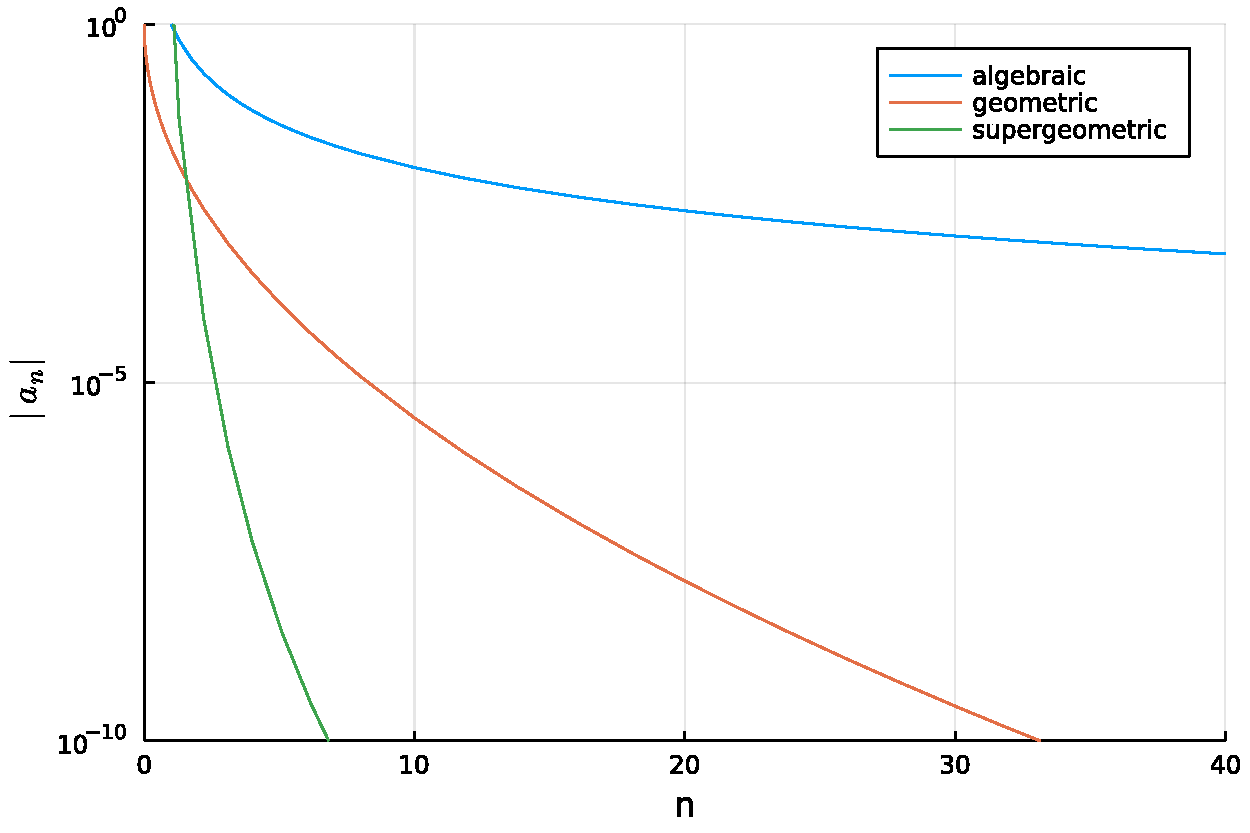
\includegraphics[keepaspectratio,scale = 0.35]{02_Fourier/typeoforder.pdf}
	\caption{Types of order}
\end{figure}

\subsubsection{その他の便利な性質}

- 微分
$$
    \frac{d}{dx} f(x) = \sum_{k=-\infty}^{\infty} (\im k)c_k e^{\im kx}
$$

- シフト
$$
    f(x-d) = \sum_{k=-\infty}^{\infty}c_ke^{\im k(x-d)} = \sum_{k=-\infty}^{\infty}(e^{-\im kd})c_ke^{\im kx}
$$

元の係数 $c_k$ に $ik$ や $e^{\im kd}$ を掛けるだけで演算ができる。
\end{comment}
%%

\subsection{フーリエ係数の計算方法}

周期関数 $f(x)$ のフーリエ係数 $c_k$ を数値計算で求めることを考える。フーリエ係数の添字のサイズ $N$ を $|k|<N$ となるように定める($N-1$ を最大波数ともいう)。

このとき、$0 = x_0\le x_1\le \dots \le x_{2N-1}=2\pi$ と区間 $[0,2\pi]$ を等間隔に分割した点 $x_j = jh$ ($j = 0,\dots,2N-1$, $h=2\pi/(2N-1)$) を標本点といい、標本点上での関数値を用いて次のようなフーリエ係数の近似を得る。

\begin{align*}
c_k &= \frac{1}{2\pi}\int_0^{2\pi}f(x)e^{-\im k x}dx \\
& \approx \frac1{2N-1}\sum_{j=0}^{2N-2} f(x_j) e^{-2\pi \im\frac{kj}{2N-1}}=\bar{c}_k,\quad (|k|<N).
\end{align*}

この $\bar{c}_k$ の式は、離散フーリエ変換の式 ($ a_k = \mathcal{F}_k(b) = \sum_{j=0}^{2M-2}b_j e^{-2\pi \im \frac{jk}{2M-1}}$) を用いて、高速フーリエ変換(FFT)で実装することができる。そして、近似されたフーリエ係数 $\bar{c}_k$ を使って、元の関数 $f(x)$ の近似が
$$
f^{(N)}(x) = \sum_{|k|<N} \bar{c}_k e^{\im k x}
$$
と得られる。

\subsection{フーリエ係数から元の関数の概形を求める}

関数 $f^{(N)}(x)$ の係数 $\bar{c}_k$ から元の関数をプロットしたい。いま標本点上での関数値は
$$
f^{(N)}(x_j) = \sum_{|k|<N} \bar{c}_k e^{\im k x_j} = \sum_{|k|<N} \bar{c}_k e^{2\pi\im \frac{kj}{2N-1}}.
$$

これは逆離散フーリエ変換に相当する。そこで逆高速フーリエ変換(IFFT)を用いて元の関数を求める。しかし、このままIFFTを用いると、標本点と同じ数の関数値しか得られず、グラフに描画すると粗くになってしまう。これを解消するために、フーリエ係数 $\bar{c}_k$ に $0$ を余分に貼り合わせて (paddingという) 、滑らかなグラフを得る。

\subsection{周期が $2\pi$ 以外の場合の取り扱い方}

$f(t)$ を周期 $L$ の周期関数とする。このとき変数 $t:a\to b$ ($L=b-a$) に対して、変数 $x$ を $x = \omega(t-a)$ ($\omega = 2\pi/L$) と定めると、$x:0\to 2\pi$ となり、関数 $g(x)\equiv f(a + \omega^{-1} x)$ は周期 $2\pi$ の周期関数である。

いま $g(x)$ がフーリエ級数
$$
g(x) = \sum_{k \in \mathbb{Z}} c_k e^{\im k x}
$$
で表されているとすると、
$$
f(t) = g(\omega (t-a)) = \sum_{k \in \mathbb{Z}} c_k e^{\im k \omega (t-a)},% = \sum_{k \in \mathbb{Z}} d_k e^{\im k \omega t},\quad d_k = e^{-\im k \omega a}c_k
$$
が成り立つ。フーリエ係数 $(c_k)_{k\in\mathbb{Z}}$ は
$$
c_k  = \frac{1}{2 \pi} \int_0 ^{2\pi} g(x) e^{-\im k x} dx = \frac{1}{L} \int_a ^b f(t) e^{-\im k \omega (t-a)} dt
$$
となり、$(c_k)_{k\in\mathbb{Z}}$ は次のように近似される。
$$
c_k \approx \frac{1}{2N-1} \sum_{j=0}^{2N-2} f(t_j) e^{-2 \pi \im \frac{kj}{2N-1}}.
$$

ここで、$t_j = a + \frac{jL}{2N-1}$ ($j=0,1,\dots,2N-2$) このことから、周期が $2\pi$ の周期関数とフーリエ係数の近似が同じ式になるため、フーリエ係数の計算方法は、先程と変わらない。

%\end{document}}
\newcommand{\Convolution}{%!TEX root = ../main.tex

%\documentclass[twoside,twocolumn,a4j,dvipdfmx]{jarticle}
%\usepackage{amsmath,amssymb}
%\usepackage[dvipdfmx]{graphicx}
%\usepackage{comment}
%\newtheorem{thm}{定理}
%\newtheorem{df}[thm]{定義}
%\newtheorem{lem}[thm]{補助定理}
%\newtheorem{prop}[thm]{補題}
%\begin{document}

\subsection{離散フーリエ変換(DFT)}
離散畳み込みを理解するための、第一歩として、離散フーリエ変換を説明する。

\begin{df} $b = (b_0, \dots , b_{2M-2}) \in \mathbb{C}^{2M-1} $ に対して、$a = \mathcal{F}(b) \in \mathbb{C}^{2M-1}$ を

$$
a_k = \mathcal{F}(b) := \sum_{j=0}^{2M-2} b_j e^{-2\pi \im (\frac{jk}{2M-1}) },\quad |k|<M
$$
とし、これを\textbf{離散フーリエ変換(DFT)}と呼ぶ。
\end{df}

\subsection{逆離散フーリエ変換(IDFT)}
\begin{df} $a = (a_{-M+1}, \dots , a_{M-1}) \in \mathbb{C}^{2M-1}$ に対して、$b = \mathcal{F}^{-1} (a) \in \mathbb{C}^{2M-1}$を
\begin{align*}
b_j &= \mathcal{F}^{-1} (a) \\
:&= \sum_{k = -M+1}^{M-1} a_k e^{2 \pi \im (\frac{jk}{2M-1})} \quad j=0, \dots , 2M-2
\end{align*}
とし、\textbf{逆離散フーリエ変換(IDFT)}と呼ぶ。
\end{df}

\textbf{注意} 一般的なDFT/IDFTはスケーリング係数をつけた形で定義されることが多い。この点で上の定義は一般的な定義と異なる。

\subsection{離散畳み込みのアルゴリズム}

今、$u_1, u_2$を周期 $L$ 、変数 $t$ に関する周期関数とし、$\omega = \frac{2\pi}{L}$とする。このとき、$u_1, u_2$をフーリエ級数展開すると、
\begin{align*}
    u_1(t) = \sum_{k \in \mathbb{Z}} a_{k}^{(1)} e^{\im k\omega t} , \quad a^{(1)} = (a_{k}^{(1)})_{k \in \mathbb{Z}} \\
    u_2(t) = \sum_{k \in \mathbb{Z}} a_{k}^{(2)} e^{\im k\omega t} , \quad a^{(2)} = (a_{k}^{(2)})_{k \in \mathbb{Z}}.
\end{align*}
そして、これらの周期関数の積は、

$$
    u_1(t)u_2(t) = \sum_{k \in \mathbb{Z}} (a^{(1)}*a^{(2)})_{k}  e^{\im k\omega t}
$$
と表される。ここで $ (a^{(1)}*a^{(2)})_k$ を\textbf{離散畳み込み}といい、
$$
     (a^{(1)}*a^{(2)})_k = \sum_{\substack{k_1 + k_2 = k \\ k_1 , k_2 \in \mathbb{Z}}} a_{k_1}^{(1)} a_{k_2}^{(2)} , \quad k \in \mathbb{Z}
$$
と表される。


さらに、数値計算への応用を意識すると、$u_1, u_2$ のような(有限モードのフーリエ級数で表される)周期関数が $p$ 個($p \in \mathbb{N}$)あったとき、
\begin{align*}
    u_i(t) &= \sum_{|k| < M} a_{k}^{(i)} e^{\im k\omega t} , \\
a^{(i)} &= (a_{k}^{(i)})_{|k| < M} \quad i = 1 , \cdots ,p \quad M \in \mathbb{Z}.
\end{align*}

離散畳み込みはこれらの周期関数の積
$$
    u_1(t)\cdots u_p(t) = \sum_{|k| \leq p(M-1)}(a^{(1)}* \cdots *a^{(p)})_k e^{\im k\omega t}
$$
を表す事になる。ここで
\begin{equation*}
    (a^{(1)}* \cdots *a^{(p)})_k = \sum_{\substack{k_1 + \cdots + k_p = k,\\ |k| \leq p(M-1),  \\ |k_1| , \cdots ,|k_p|<M}} a_{k_1}^{(1)} \cdots  a_{k_p}^{(p)} 
\end{equation*}
と表される。

\subsubsection{畳み込みの定理}
畳み込みを離散フーリエ変換したものは、それぞれのフーリエ係数の離散フーリエ変換の積になる。
$$
\begin{aligned}
    \mathcal{F}(a^{(1)}* \cdots *a^{(p)}) &= \mathcal{F}(a^{(1)})\hat{\ast} \cdots \hat{\ast}\mathcal{F}(a^{(p)}) \\
    &= b^{(1)}\hat{\ast}\cdots \hat{\ast}b^{(p)} .
\end{aligned}
$$
ここで $ b^{(1)}\hat{\ast} \cdots \hat{\ast}b^{(p)}$ におけるベクトル同士の積は、要素毎の積を表す。

\subsubsection{離散フーリエ変換を使った畳み込みの計算方法(FFTアルゴリズム)\cite{convolution} }

実際の畳み込みの計算方法について説明する。
周期$L$、変数$t$の周期関数 $u_i(t)$ が有限項のフーリエ級数
$$
    u_i(t) = \sum_{|k|<M} a_{k}^{(i)} e^{\im k\omega t} , \quad a^{(i)} = (a_{k}^{(i)})_{|k|<M} 
$$
で表されているとする。ここで $\omega = \frac{2 \pi}{L}$ とする。このとき、$p$ 個の関数の積
$$
    u_1(t)\cdots u_p(t) = \sum_{|k| \leq p(M-1)}c_k e^{\im k\omega t}
$$
を表現するフーリエ係数 $(c_k)_{|k| \leq p(M-1)}$ を以下の計算方法により求める。

\textbf{入力}: $a^{(i)} = (a^{(i)}_k)_{|k|<M}\in\mathbb{C}^{2M-1} \quad (i = 1, \cdots , p)$

\textbf{Step1}: エイリアシングエラーを防ぐために、入力された値 $a^{(i)}$ の両脇に $(p-1)M$ 個の $0$ を付け加える。これを $\tilde{a}^{(i)}$ と書く。

\footnotesize
$$
    \tilde{a}^{(i)} = (\underbrace{0, \cdots , 0}_{(p-1)M\text{個}}, \underbrace{a^{(i)}_{-M+1}, \cdots , a^{(i)}_{M-1}}_{2M-1\text{個}},\underbrace{0, \cdots , 0}_{(p-1)M\text{個}}) \in \mathbb{C}^{2pM-1}
$$
\normalsize

\textbf{Step2}: step1で得た値 $\tilde{a}^{(i)}$ に対して逆離散フーリエ変換を行う。変換した後の値を $\tilde{b}^{(i)}$ と置く。
$$
    \tilde{b}^{(i)} = \mathcal{F}^{-1}(\tilde{a}^{(i)}) \in \mathbb{C}^{2pM-1}
$$

\textbf{Step3}: $ (\tilde{b}^{(1)} \hat{*} \cdots \hat{*} \tilde{b}^{(p)}) $を計算する。上記の畳み込みの定理と同じく、このベクトル同士の積は、要素毎の積を表す。
$$
    (\tilde{b}^{(1)} \hat{*} \cdots \hat{*} \tilde{b}^{(p)} )_{j} = \tilde{b}^{(1)}_j \cdots \tilde{b}^{(p)}_j , \quad j = 0, \cdots , 2pM-2
$$

\textbf{Step4}: step3で求めた$ (\tilde{b}^{(1)} \hat{*} \cdots \hat{*} \tilde{b}^{(p)}) $に対して、離散フーリエ変換を行い、得た値を $2pM-1$ で割る。
$$
     c_k = \frac{1}{2pM-1} \mathcal{F}_k (\tilde{b}^{(i)} \tilde{*} \cdots \tilde{*} \tilde{b}^{(p)}) \quad |k| \leq p(M-1)
$$

求めた $c_k$ のうち、実際に必要なのは両脇の $p-1$ 個を取り除いた $|k| \leq p(M-1)$ 個である。
\footnotesize
$$
    c = (\underbrace{0, \cdots , 0}_{(p-1)M\text{個}}, \underbrace{a^{(i)}_{-M+1}, \cdots , a^{(i)}_{M-1}}_{2M-1\text{個}},\underbrace{0, \cdots , 0}_{(p-1)M\text{個}}) \in \mathbb{C}^{2pM-1}
$$
\normalsize


\textbf{出力}:$c = (c_k)_{|k|\le p(M-1)}\in\mathbb{C}^{2p(M-1)+1}$

%---------------------------------------------------------------
%具体例なので省略
\begin{comment}
\subsubsection{具体例}
周期関数を $f(x)=\frac{\exp(\sin(5x))}{1+\sin(\cos(x))}$ と決めて、畳み込みを行う。


\begin{verbatim}
#f(x)の概形

f(x) = exp(sin(5x))/(1+sin(cos(x)))
plot(f,0,2π)
\end{verbatim}

\begin{figure}[h]
	\centering
	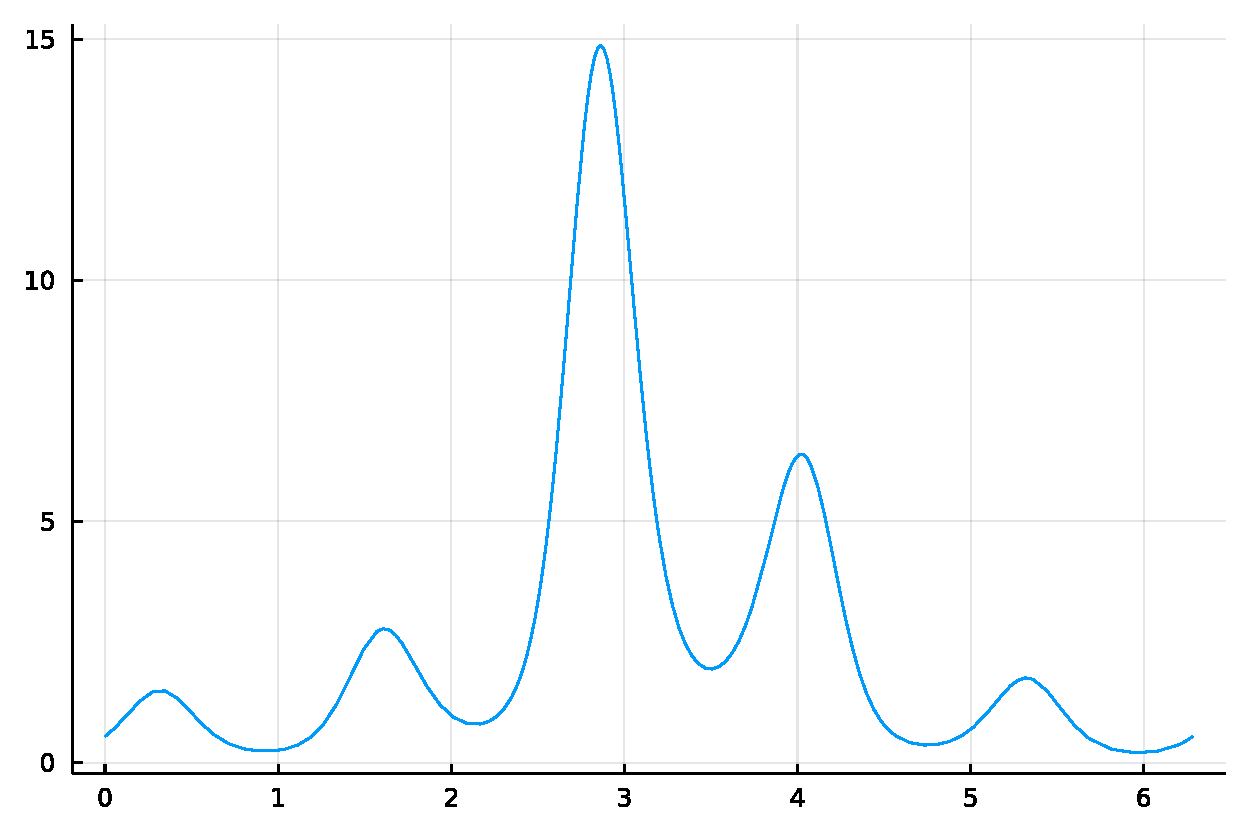
\includegraphics[keepaspectratio,scale = 0.4]{Plot_f(x).pdf}
	\caption{Plot $f(x)$}
\end{figure}

\texttt{ApproxFun.jl}で $f(x)$ を近似してみると、グラフは下のようになる。

\begin{verbatim}
using ApproxFun, FFTW
fc = Fun(f,Laurent())
plot(real(fc))
\end{verbatim}

\begin{figure}[h]
	\centering
	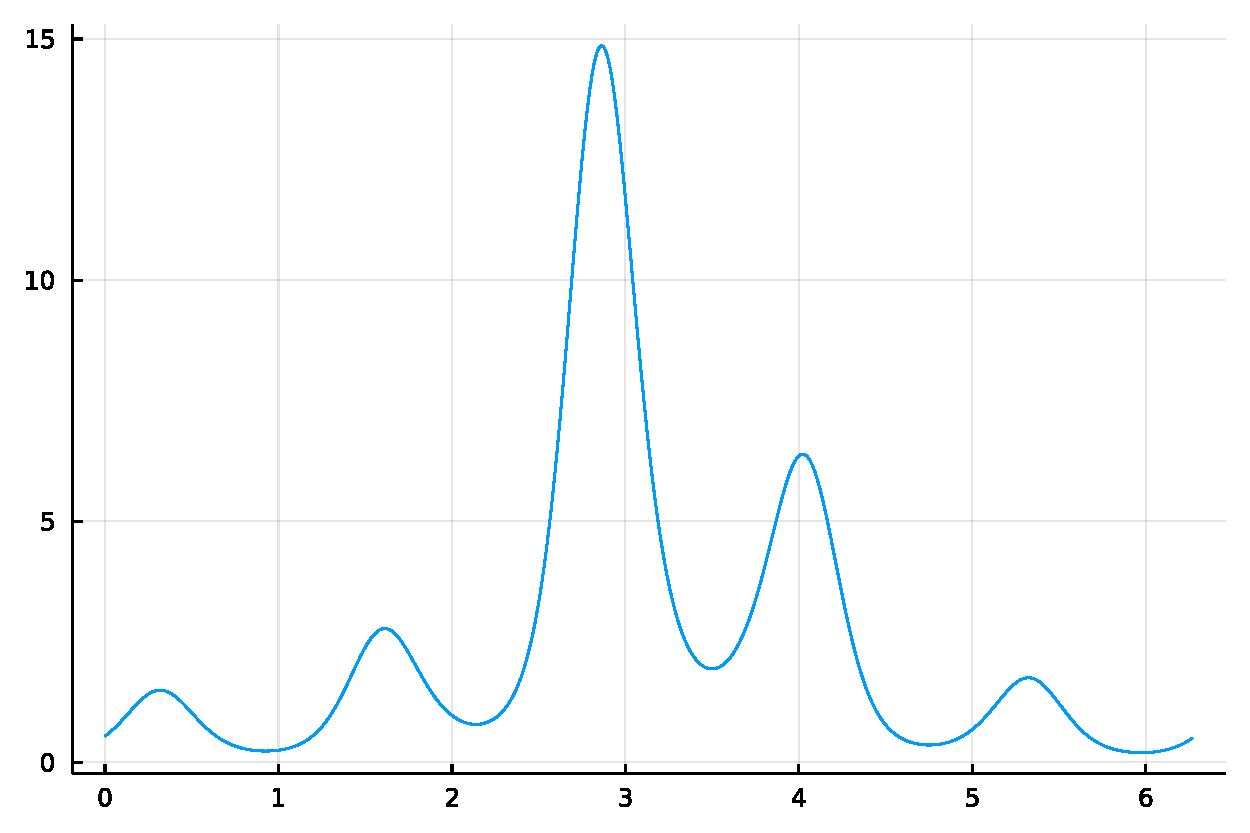
\includegraphics[keepaspectratio,scale = 0.4]{Plot_f(x)_approxfun.pdf}
	\caption{Plot $f(x)$ of \texttt{ApproxFun.jl}}
\end{figure}

フーリエ係数を比較すると一致することが確認できる。

\footnotesize
\begin{verbatim}
m = ncoefficients(fc)
M = Int((m+1)/2)
c = coefficients(fc) # coefficients of ApproxFun
function index_shift(c) # convert c -> fourier coeffs
    return [reverse(c[2:2:end]);c[1:2:end]]
end
a = fouriercoeffs(f,M) 
plot(abs.(a),yscale=:log10,label="computed via FFT")
plot!(abs.(index_shift(c)),yscale=:log10,label = "ApproxFun")
\end{verbatim}
\normalsize

\begin{figure}[h]
	\centering
	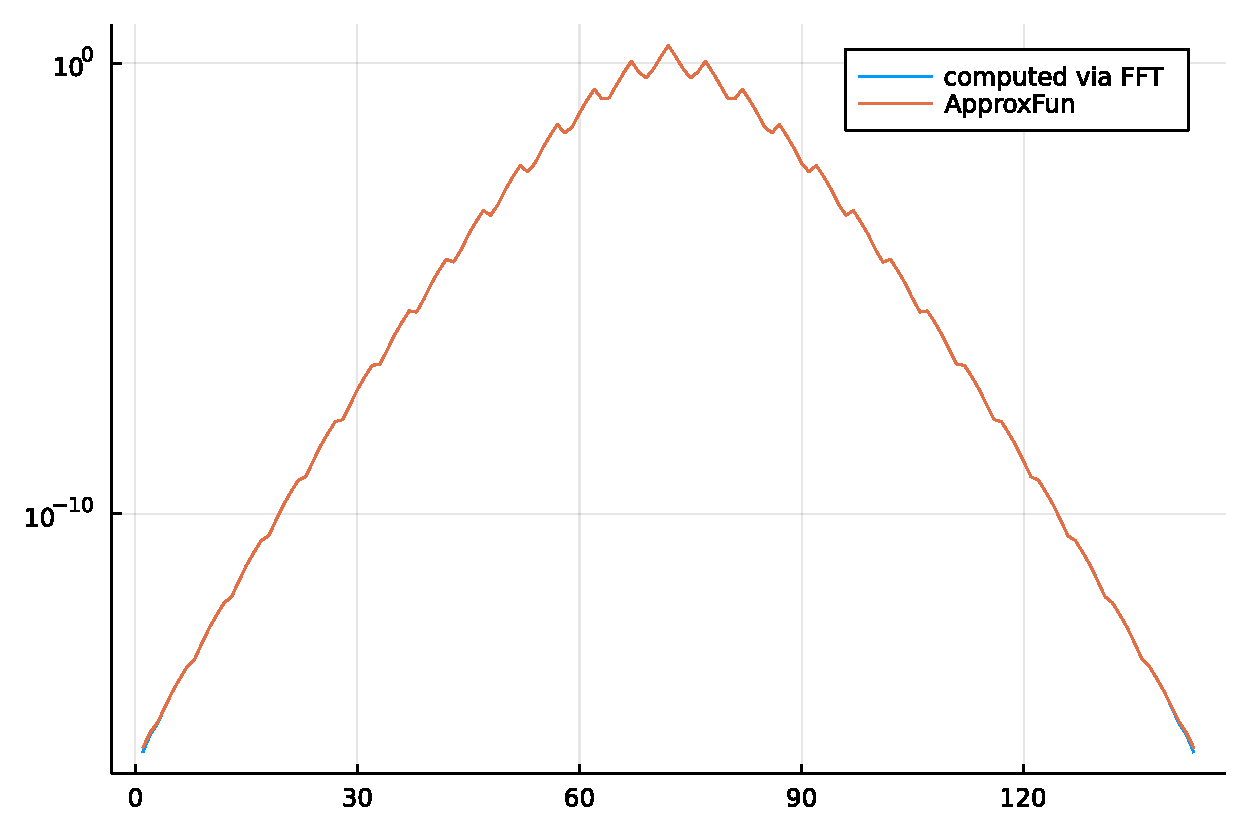
\includegraphics[keepaspectratio,scale = 0.4]{compare_coeffs_FFT_approxfun.pdf}
	\caption{coefficients of FFT and \texttt{ApproxFun.jl}}
\end{figure}

この周期関数の2乗をする場合の畳み込みについて考えてみよう。2乗した関数の概形は、

\begin{verbatim}
plot(real(fc)^2)
\end{verbatim}

\begin{figure}[h]
	\centering
	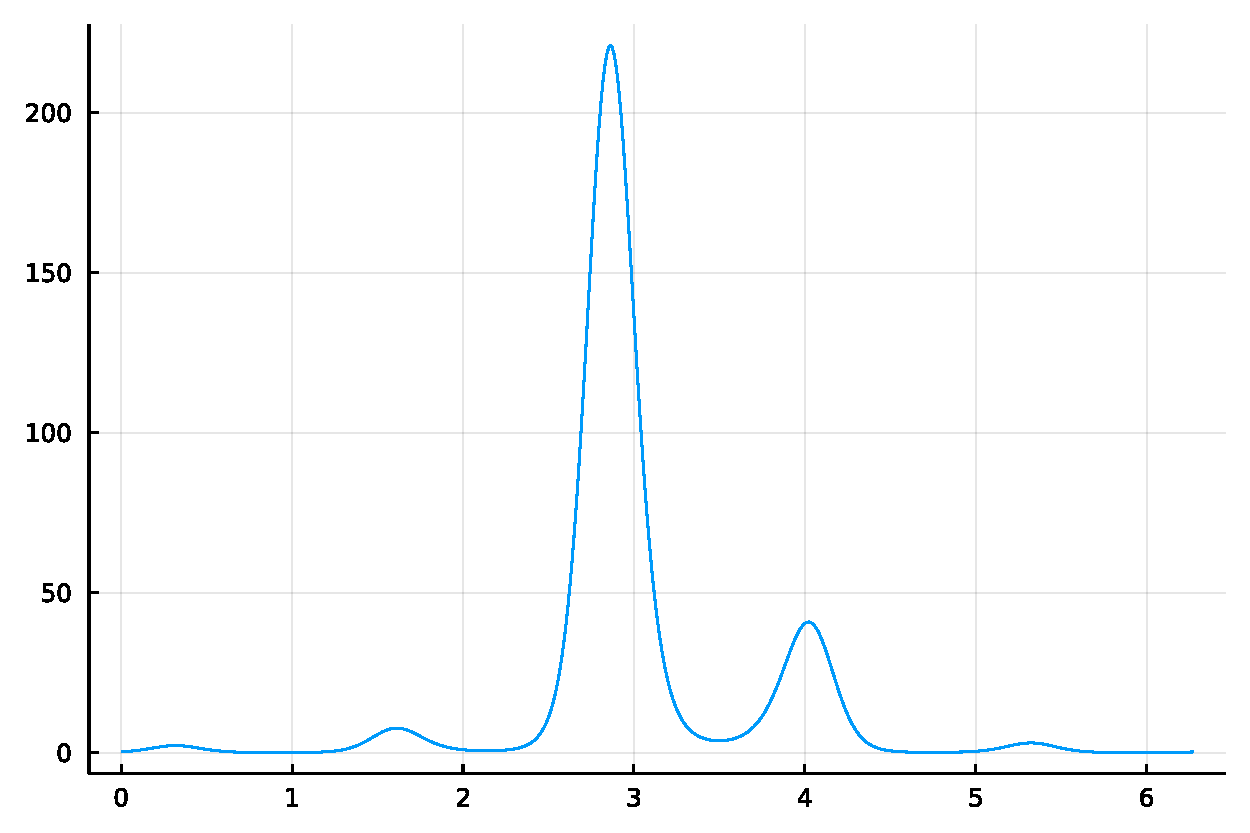
\includegraphics[keepaspectratio,scale = 0.4]{Plot_f(x)^2.pdf}
	\caption{Plot $f(x)^2$}
\end{figure}

一方、FFTアルゴリズムを用いて2乗した関数のフーリエ係数を求め、得たフーリエ級数の概形をプロットすると次のようになる。

\footnotesize
\begin{verbatim}
# FFT Algorithm
p = 2
N = (p-1)*M
ta = [zeros(N,1);a;zeros(N,1)] # 1. Padding zeros
tb = ifft(ifftshift(ta)) # 2. IFFT of ta
tb^p = tb.^p # 3. tb*^tb

# 4. FFT of tb2 
c^p = fftshift(fft(tb^p))*(2.0*p*M-1)^(p-1) 

plot_fourier!(c^p)
\end{verbatim}
\normalsize

\begin{figure}[h]
	\centering
	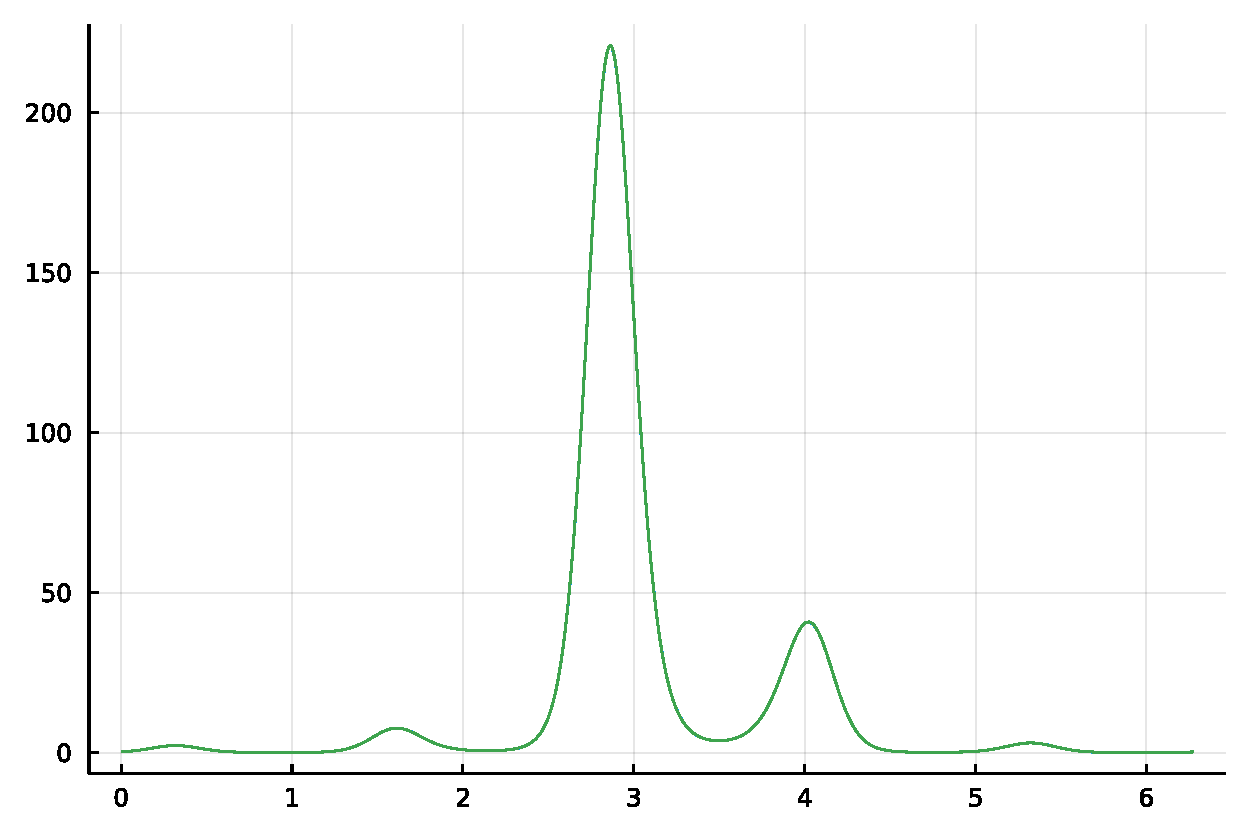
\includegraphics[keepaspectratio,scale = 0.4]{Plot_f(x)_FFT.pdf}
	\caption{Plot $f(x)^2$ and $f(x)^2$ of FFT}
\end{figure}

二つの概形が一致しているのが分かる(水色と赤の曲線がほぼ一致している)。次に、このプログラムを関数化してみよう。

関数が与えられたら、そのフーリエ係数を計算する\texttt{fouriercoeffs}を使って得たフーリエ係数の離散畳み込み(\texttt{powerconvfourier})を計算することで、関数の冪乗を計算できる。
\end{comment}
%---------------------------------------------------------------

\begin{comment}
下記のコードが離散畳み込みを実装した関数になる。また、本論文に記載されているコードは、2段組の都合上、適宜改行されている。

\footnotesize
\begin{verbatim}
function powerconvfourier(a::Vector{Complex{T}}
                                     ,p) where T
    M = Int((length(a)+1)/2)
    N = (p-1)*M

    # 1. Padding zeros: size(ta) = 2pM-1
    ta = [zeros(N,1);a;zeros(N,1)] 

    # 2. IFFT of ta
    tb = ifft(ifftshift(ta)) 
    tb^p = tb.^p # 3. tb*^tb
    c^p = fftshift(fft(tb^p))*(2.0*p*M-1)^(p-1)

    # return (truncated, full) version
    return c^p[N+1:end-N], c^p[p:end-(p-1)]
end
\end{verbatim}
\normalsize

\subsection{離散畳み込みの精度保証付き数値計算}
離散畳み込みの精度保証を行う。離散畳み込みのアルゴリズムには、FFTが含まれるため、まず、FFTの精度保証を行うための関数を定義する。コードについては付録に記載する。
\end{comment}

%---------------------------------------------------------------
\begin{comment}
\begin{verbatim}
M = 150
p = 2
f(x) = erf(sin(3x)+cos(2x))^4
g(x) = f(x)^p

a = fouriercoeffs(f,M) # size(a) = 2M-1
# plot(abs.(a),yscale=:log10,)

ia = map(Interval, a)

length_ia = 2M-1
length_ia_ext = nextpow(2,length_ia)
n = Int((length_ia_ext - length_ia + 1)/2) # 2n-1
ia_ext = map(Interval,im*zeros(length_ia_ext))
ia_ext[n+1:end-n+1] = ia
verifyfft(ia_ext,1)# sign = 1(fft), -1(ifft)
\end{verbatim}
\end{comment}
%---------------------------------------------------------------

\begin{comment}

\texttt{verifyfft}は、要素数が2のべき乗の場合しか実行できないので、step1のpaddingの部分で要素数を調整する。
\begin{align*}
\tilde{a}=(&\underbrace{0, \cdots , 0}_{L\text{個}},\underbrace{0, \cdots , 0}_{N=(p-1)M\text{個}}, \underbrace{a_{-M+1}, \cdots , a_{M-1}}_{2M-1\text{個}}, \\
&\underbrace{0, \cdots , 0}_{N\text{個}},\underbrace{0, \cdots , 0}_{L-1\text{個}}) \in \mathbb{C}^{2pM-2+2L}
\end{align*}

\begin{align*}
c=(&\underbrace{0, \cdots , 0}_{L\text{個}},\underbrace{0, \cdots , 0}_{(p-1)\text{個}}, \underbrace{a_{-p(M-1)}, \cdots , a_{p(M-1)}}_{2p(M-1)+1\text{個}},\\
&\underbrace{0, \cdots , 0}_{(p-1)\text{個}},\underbrace{0, \cdots , 0}_{L-1\text{個}}) \in \mathbb{C}^{2pM-2+2L}
\end{align*}

%step1の \texttt{ia\_ext} が上の $\tilde{a}$ を指し、\texttt{ic\_ext} が $c$ である。2のべき乗になるようにpaddingした分、関数の最後に取り出す値の範囲に注意する。
下記のコードは、区間演算とベクトル、両方の型に対応できるように、多重ディスパッチを利用する離散畳み込みの関数である。

\footnotesize
\begin{verbatim}
function powerconvfourier(a::Vector{Complex{Interval{T}}}
                                     ,p) where T
    M = Int((length(a)+1)/2) # length(a) = 2M-1
    N = (p-1)*M
    ia = map(Interval, a)

    length_ia = 2*p*M-1
    length_ia_ext = nextpow(2,length_ia)# 2pM-2+2L
    
    L = Int((length_ia_ext - length_ia + 1)/2)
    
    # step.1 : padding (p-1)M + L zeros for each sides
    ia_ext = map(Complex{Interval},zeros(length_ia_ext))
    ia_ext[L+N+1:end-L-N+1] = ia  #\tilda{a}

    # step.2 : inverse fft
    #sign = -1 : ifft
    ib_ext = verifyfft(ifftshift(ia_ext), -1) 
    
    # step.3 : power p elementwisely
    ib_ext^p = ib_ext.^p
    
    # step.4 : fft with rescaling
    #sign = 1 : fft
    ic_ext^p = fftshift(verifyfft(ib_ext^p, 1)) 
                  * length_ia_ext^(p-1)  
    
    # return ic_ext^p,ic_ext^p
    # return (truncated, full) version
    return ic_ext^p[L+N+1:end-N-L+1]
                         , ic_ext^p[L+p:end-(L+p-2)] 
end
\end{verbatim}
\normalsize
\end{comment}

%---------------------------------------------------------------
\begin{comment}
\begin{verbatim}
c,c_full = powerconvfourier(a,2);
ic,ic_full = powerconvfourier(ia,2);# 多重ディスパッチ
\end{verbatim}

区間演算は、数値計算で得た値の範囲全体を含むため、\texttt{ic\_full $\in$ c\_full}が成り立つ。

また、下の図からテイルに$10^{-15}$ほどの誤差が含まれていることがわかる。

\begin{verbatim}
using IntervalArithmetic:mid
@show c_full .∈ ic_full
plot(abs.(c_full),yscale=:log10,label="non-rigorous")
plot!(mid.(abs.(ic_full)),yscale=:log10,label="rigorous")
\end{verbatim}
\end{comment}
%---------------------------------------------------------------

%\end{document}}
\newcommand{\Theories}{%!TEX root = ../main.tex

%\documentclass[twoside,twocolumn,a4j,dvipdfmx]{jarticle}
%\usepackage{amsmath,amssymb}
%\usepackage[dvipdfmx]{graphicx}
%\newcommand{\im}{\mathrm{i}}
%\newcommand{\bx}{\mathrm x}
%\newcommand{\R}{\mathbb{R}}
%\newtheorem{thm}{定理}[section]
%\newtheorem{df}[thm]{定義}
%\newtheorem{lem}{補助定理}[section]
%\newtheorem{prop}{補題}[section]

%\begin{document}

\subsection{ノルム空間、Banach空間、距離空間}

\begin{df}
線形空間(ベクトル空間)とは和(と差)、スカラー倍が定義される集合、特に $X$ をある集合として、
\begin{itemize}
\item 和の演算が可換 : $(x+y)+z = x+(y+z), \forall x,y,z \in X$
\item ゼロ元が存在 : $\exists0 \in X \mbox{ such that } 0 + v = v$ 
\end{itemize}
である。
\end{df}

\begin{df}
線形空間 $X$ の各元に実数値を対応させる関数 $\|\cdot\| : X \rightarrow \R$ が定義され、\textbf{ノルムの公理}
\begin{enumerate}
\item $\|x\| \ge 0 \mbox{、かつ} \|x\| = 0 \Leftrightarrow x = 0,x \in X$
\item $\|cx\| = |c|\|x\|, c \in \R, x \in X$
\item $\|x+y\| \leq \|x\| + \|y\|, x,y \in X$
\end{enumerate}
を満たすとき、 $X$ を\textbf{ノルム空間} という。
\end{df}

ノルム空間が\textbf{完備}とは、 $X$ の任意のCauchy列 $\{ x_n \}$ が $X$ のある元 $x_*$ に収束する, i.e, $\exists x_* \in X \mbox{ such that } x_n \Rightarrow x_* \mbox{ as } n \Rightarrow \infty \Leftrightarrow \|x_n - x_* \| \Rightarrow 0  \mbox{ as } n \Rightarrow \infty$

\begin{df}
完備なノルム空間を\textbf{Banach空間}という
\end{df}

\begin{df}
$X$ をノルム空間とし、 $x,y \in X$ に対して実数値を対応させる関数 $d(\cdot, \cdot) :X \times X \to \R$ が定義され、条件
\begin{enumerate}
\item $d(x,y) \ge 0$, かつ $d(x,y) = 0 \Leftrightarrow x = y, \quad x,y \in X$
\item $d(x,y) = d(y,x), \quad x,y \in X$
\item $d(x,y) \leq d(x,z) + d(z,y) \quad x,y,z \in X$
\end{enumerate}
を満たすとき、 $d$ を距離という、距離の備わっている集合を\textbf{距離空間}という。
\end{df}

\subsection{Banachの不動点定理(縮小写像の原理)}
\begin{df}
$(X,d)$ : 距離空間, $T:X \to X$ が $X$ 上の縮小写像である必要十分条件は、$d(T(x),T(y)) \leq kd(x,y), \quad x,y \in X$ となるような $k \in [0,1) $ が存在することである。
\end{df}

\begin{thm}[Banachの不動点定理]
$(X,d)$ : 完備距離空間とする。写像 $T: X \to X$ が縮小写像ならば、 $T$ は $X$ においてただ一つの不動点 $x_* = T(x_*)$ をもつ。
\end{thm}

\subsection{簡易ニュートン写像}

\begin{df}  $X$, $Y$ をBanach空間とし, 写像 $F:X\rightarrow Y$ に対して, 
$$
F(\bx)=0 \quad \text{in}~Y
$$
という(非線形)作用素方程式を考える。
このとき写像 $T:X\rightarrow X$ を
$$
T(\bx):=\bx-AF(\bx)
$$
と定義したとき, これを\textbf{簡易ニュートン写像}という。ここで,  $A:Y\rightarrow X$ はある全単射な線形作用素である。このとき, $\bar{\bx}$を $F(\bar{\bx}) \approx 0$ の近似解とし, $\bar{x}$ の近傍を
$$
\begin{array}{ll}
B(\bar{\bx}, r):=\{\bx \in X:\|\bx-\bar{\bx}\|<r\} & \text { (開球) } \\
\overline{B(\bar{\bx}, r)}:=\{\bx \in X:\|\bx-\bar{\bx}\| \leq r\} & \text { (閉球) }
\end{array}
$$
で定義する。このときもし, $B(\bar{\bx}, r)$ 上で写像 $T$ が縮小写像となれば, Banachの不動点定理から $F(\bar{\bx})=0$をみたす解 $\tilde{\bx} \in B(\bar{\bx}, r)$がただ1つ存在することになる。

このように解の存在を仮定せずに近似解近傍での収束をいう定理を Newton 法の半局所的収束定理という。
\end{df}

\subsection{有界線形作用素}
\begin{df}
Banach空間 $X$ から $Y$への有界線形作用素全体を
\begin{align*}
 \mathcal{L}(X, Y):=\{&E:X\rightarrow Y:E\text{が線形},\\
&\|E\|_{ \mathcal{L}(X, Y)}<\infty \}
\end{align*}
とする。ここで $\|\cdot\|_{ \mathcal{L}(X, Y)}$ は作用素ノルム
$$
\|E\|_{\mathcal{L}(X, Y)}:=\sup _{\|\bx\|_{X}=1}\|E \bx\|_{Y}
$$

を表す。そして空間 $\left\langle\mathcal{L}(X, Y),\|\cdot\|_{\mathcal{L}(X, Y)}\right\rangle$ はBanach空間となる。
\end{df}

\subsection{Fréchet微分}
\begin{df}
作用素 $F:X\rightarrow Y$が $\bx_0 \in X$ でFréchet微分可能であるとは, ある有界線形作用素 $E:X \rightarrow Y$ が存在して, 
$$
\lim _{\|h\|_{X} \rightarrow 0} \frac{\left\|F\left(\bx_{0}+h\right) - F\left(\bx_{0}\right)-E h\right\|_{Y}}{\|h\|_{X}}=0
$$
が成り立つことをいう。このとき, $E$ は作用素 $F$ の $\bx_0$ におけるFréchet微分といい, $E=DF(\bx_0)$ とかく。 もしも作用素 $F:X\rightarrow Y$ がすべての $\bx\in X$ に対してFréchet微分可能ならば, $F$ は $X$ において $C^1$-Fréchet微分可能という。
\end{df}

\subsection{許容重み}

\begin{df}点列 $w = (w_k)_{k \in \mathbb{Z}}$ について、
\begin{align*}
    w_k > 0 \quad (\forall k \in \mathbb{Z}) \\
    w_{n+k} \leq w_n w_k \quad ( \forall n,k \in \mathbb{Z})
\end{align*}
が成立するとき、許容重みであるという。
\end{df}

\begin{example}
$s>0, \nu \leq 1$ に対して、
$$
    w_k = (1 + |k|)^s \nu^{|k|} , \quad k \in \mathbb{Z}
$$
と定義される $w_k$ は許容重みである。この許容重みであるような点列 $w_k$ に対して、次のような重み付き $\ell^1$ 空間が定義できる。
\footnotesize
\begin{align*}
     \ell^1_w := \left\{ a = (a_k)_{k \in \mathbb{Z}}: a_k \in \mathbb{C}, \| a \|_w := \sum_{k \in \mathbb{Z} }|a_k | w_k < \infty \right\}.
\end{align*}
\end{example}
\normalsize

\subsection{Newton-Kantrovich 型定理}
\begin{thm}
$X$, $Y$ をBanach空間、$\mathcal{L}(X,Y)$ を $X$ から $Y$ への有界線形作用素全体の集合とする。有界線形作用素 $A^\dagger \in \mathcal{L}(X,Y)$, $A \in \mathcal{L} (Y,X)$ を考え、作用素 $F: X \rightarrow Y$ が $C^1$-Fréchet微分可能とする。また $A$ が単射で $AF: X \rightarrow X$ とする。いま、$\bar \bx \in X$に対して、正定数 $Y_0$, $Z_0$, $Z_1$, および非減少関数 $Z_2(r)$ ($r>0$) が存在して、次の不等式
    \begin{align*}
    \|AF(\bar \bx)\|_X &\leq Y_0 \\
    \|I - A A^\dagger\|_{\mathcal{L}(X)} &\leq Z_0 \\
    \|A (DF(\bar \bx) - A^\dagger)\|_{\mathcal{L}(X)}&\leq Z_1 \\
    \|A (DF(b) - DF(\bar \bx))\|_{\mathcal{L}(X)} &\leq Z_2 (r)r, \\
    \forall b &\in \overline{B(\bar \bx, r)}
    \end{align*}
をみたすとする。このとき、radii polynomialを以下で定義する。
$$
    p(r) := Z_2 (r)r^2 - (1 - Z_1 - Z_0)r + Y_0.
$$

これに対し、$p(r_0)<0$ となる $r_0 > 0$ が存在すれば、$F(\bx) = 0$ をみたす解 $\tilde \bx$ が $b \in \overline{B(\bar \bx, r)}$ 内に一意存在する。
\end{thm}

Newton-Kantorovich型定理を利用する数値検証の際には、$DF(\bar \bx)$ を $F$ の $\bar \bx$ におけるFréchet微分、$A^\dagger$ を $DF(\bar \bx)$ の近似、$A$ を $A^\dagger$ の近似左逆作用素とする。($AA^\dagger \approx I$ とするのが一般的である。)

\subsection{Newton法}
まず、1次元のNewton法を考える。$f: \R \to \R, x \in \R$ として
$$
f(x) = 0
$$
となる $x$ を求める。このとき、 $x$ の付近に適当な値 $x_0$ をとり、次の漸化式によって $x$ に収束する数列を得ることができる。
$$
x_{n+1} = x_n - \frac{f(x_n)}{f'(x_n)}
$$

本研究では、多次元のNewton法を用いる。 $F(x_n) \in \R^{2N} \to \R^{2N}$ とし、 $F'$ の代わりにヤコビ行列 $DF$ を用いて次で表される。
\begin{align*}
x_{n+1} = x_n - DF(x_n)^{-1}F(x_n), \\
DF(x) = 
\begin{bmatrix}
\frac{\partial F_1}{\partial x_1} & \cdots & \frac{\partial F_1}{\partial x_{2N}} \\
\vdots & & \vdots \\
\frac{\partial F_{2N}}{\partial x_1}  & \cdots & \frac{\partial F_{2N}}{\partial x_{2N}} 
\end{bmatrix}
\end{align*}

\subsection{Krawczyk (クラフチック) 法}
\begin{thm}
$X \in \mathbb{IR}^N$ をベクトル区間(候補集合ともいう)、 $c = \opmid(X), R \simeq Df(c)^{-1} = J(c)^{-1}, E$ を単位行列とし、
$$
    K(X) = c - Rf(c) + (E - RDf(X))(X-c)
$$
としたとき、 $K(X) \subset \opint(X) (\opint(X) : X$ の内部) ならば $X$ に $f(x) = 0$ の解が唯一存在する。
\end{thm}

\subsection{Banach空間 $X$ の設定}

本研究で用いるBanach空間$X$を次のように定める。はじめに重み付き $\ell^1$ 空間を重み $w_k=\nu^{|k|}$ (今は$\nu=1.1$) として次のように定める。
\footnotesize
\begin{align*}
\ell^1_\nu := &\left\{ a = (a_k)_{k \in \mathbb{Z}}: a_k \in \mathbb{C}, \| a \|_w := \sum_{k \in \mathbb{Z} }|a_k | \nu^{|k|} < \infty \right\}.
\end{align*}
\normalsize
そして、関数空間 $X$ は
$$
    X := \mathbb{C} \times \ell^1_{\nu}, \quad \bx = (\omega, a), \quad \omega \in \mathbb{C}, \quad a \in \ell^1_\nu
$$
と定め、そのノルムを
$$
    \| \bx \|_X := \max\{ |\omega|, \| a \|_w \}
$$
として定義する。このとき、$X$ はBanach空間となる。



%\end{document}}
\newcommand{\ODE}{%!TEX root = ../main.tex

%\documentclass[twoside,twocolumn,a4j,dvipdfmx]{jarticle}
%\usepackage{amsmath,amssymb}
%\usepackage[dvipdfmx]{graphicx}
%\newcommand{\im}{\mathrm{i}}
%\newcommand{\bx}{\mathrm x}
%\begin{document}

常微分方程式の一つであるvan der Pol方程式の周期解の数値計算をまず行い、得た近似解をもとに解の精度保証を行う。

\subsection{van der Pol 方程式}
van der Pol方程式とは、以下のような方程式である。
$$
\frac{d^2 x}{dt^2} - \mu (1-x^2)\frac{dx}{dt} + x = 0.
$$
ここで、$x(t)$ が未知関数で、$\mu>0$ は非線形の減衰の強さを表すパラメータである。van der Pol 方程式を次の連立常微分方程式系にして\texttt{DifferentialEquations.jl}のというJulia言語のパッケージ\cite{DEjl}に実装されているODEソルバーで数値計算する。
$$
\begin{cases}
\dot{x} = y\\
\dot{y} = \mu (1-x^2)y - x.
\end{cases}
$$
初期値は $x(0)=0$, $y(0)=2$とし, $\mu=1$ とする。

%%
\begin{comment}
\begin{verbatim}
using DifferentialEquations

function vanderpol(du, u , μ ,t)
    x,y = u
    du[1] = y
    du[2] = μ*(1- x ^2)*y - x
end

u0 = [0.0; 2.0]
tspan = (0.0, 300)
μ = 1.0
prob = ODEProblem(vanderpol, u0, tspan, μ)
sol = solve(prob,Tsit5(),
           reltol=1e-8,abstol=1e-8)
\end{verbatim}
\end{comment}

\begin{comment}
\subsection{Newton法の初期値の設定}

まず、フーリエ級数の係数を求めるために、van der Pol方程式の周期解の周期を大まかに求める。

\begin{verbatim}
a = 30
app_period = 6.55
timestep = 0.1

f_tmp = sol(a+app_period/2:timestep:a
               +3*app_period/2)
find_period = abs.(f_tmp .- sol(a))
(~,ind) = findmin(find_period[1,:])
b = a+app_period/2 + timestep*(ind-1)
\end{verbatim}
\end{comment}
%%

\subsection{Newton法を用いた周期解の求め方}

van der Pol方程式は、$\dot{x} = \frac{dx}{dt}$とおくと、以下のように表すことができる。
$$
\ddot{x} - \mu(1-x^2)\dot{x} + x = 0.
$$
後の計算のために、式を少し整理すると、
$$
\ddot{x} - \mu\dot{x} + \frac{\mu}{3} \dot{(x^3)} + x = 0
$$
と書ける。また、周期解$x(t)$を周期$L$の周期関数とし、$\omega = \frac{2\pi}{L}$とおくと、$x(t)$とその微分や$2$乗はフーリエ級数を使って、
\begin{align*}
x(t) &= \sum_{k \in \mathbb{Z}} a_k e^{\im k\omega t}\\
\frac{dx(t)}{dt} &= \sum_{k \in \mathbb{Z}}(\im k \omega) a_k e^{\im k \omega t} \\
\frac{d^2 x(t)}{dt^2} &= \sum_{k \in \mathbb{Z}} (-  k^2 \omega^2 )a_k e^{\im k\omega t} \\
x(t)^3 &= \sum_{k \in \mathbb{Z}} (a * a * a)_k e^{\im k \omega t}
\end{align*}
と書くことができる。ここで
\begin{equation*}
(a^3)_k := \sum_{\substack{k_1+k_2+k_3 = k\\k_i\in\mathbb{Z}}} a_{k_1}a_{k_2}
a_{k_3},\quad k\in\mathbb{Z}
\end{equation*}
は3次の離散たたみこみである。

以上の式を用いて、フーリエ係数に関する式を立てる。$a = (a_k)_{k \in \mathbb{Z}}$に対して、van der Pol方程式に求めたフーリエ級数を代入すると、
$$
f_k(a) := -k^2\omega^2 a_k - \mu\im k \omega a_k + \frac{\mu }{3}(\im k \omega)(a*a*a)_k + a_k
$$
となる点列 $\left(f_k(a)\right)_{k\in\mathbb{Z}}$が得られる。そして、点列 $a$ がvan der Pol方程式の解のフーリエ係数になっているならば、各 $k\in\mathbb{Z}$ について
$$
f_k(a) = 0
$$
となる。このときの未知数は周波数 $\omega$ と点列 $a$ であり、これらを並べて $\bx = (\omega,a)$ と書くことにする。未知数 $\bx$ に対して、$f_k(a) = 0$ という方程式だけでは不定な方程式になるため、解の形を一つに定める事ができない。そこで、位相条件
\begin{equation*}
    \eta (a) := \sum_{|k|<N} a_k - \eta_0=0, \quad \eta_0 \in \mathbb{R} 
\end{equation*}
を加える。この条件は $x(t)$ の初期値 $x(0) = \eta_0$ を表している。最終的に van der Pol 方程式の周期解の求解は次の代数方程式を解くことに帰着される。
$$
    F(\bx) := 
    \begin{bmatrix}
    \eta (a) \\
    (f_k(a)_{k\in\mathbb{Z}}
    \end{bmatrix}
    =0.
$$

以下、この零点探索問題 $F(\bx)=0$ について Newton 法で解を得ることを考える。まず $N$ をフーリエ係数の打ち切り番号(最大波数:$N-1$)とし、周期解の近似を次のように構成する。
$$
 \bar{x}(t) = \sum_{|k|<N} \bar{a}_k e^{\im k \bar\omega t}.
$$

このとき、フーリエ係数と(近似)周期を並べた
$$
    \bar{\bx} = (\bar\omega, \bar{a}_{-N+1},\dots,\bar{a}_{N-1})\in \mathbb{C}^{2N}
$$
を近似解とよぶ。近似解 $\bar \bx$ の未知数は $2N$ 個。そして $f_k(a)=0$ を $|k|<N$ の範囲で打ち切る方程式
$$
    F^{(N)}(\bx^{(N)}) = 
    \begin{bmatrix}
    \eta (a^{(N)}) \\
    (f_k(a^{(N)}))_{k < |N|}
    \end{bmatrix}
    =0
$$
を考える。ここで $a^{(N)} = (a_k)_{|k|<N}$, $\bx^{(N)} = (\omega,a^{(N)})$ をそれぞれ表し、$F^{(N)}:\mathbb{C}^{2N}\to \mathbb{C}^{2N}$ である。したがって $F^{(N)}(\bx^{(N)}) = 0$ という有限次元の非線形方程式を解くことで、近似解 $\bar \bx$ が得られる。

\subsection{Newton法による周期解の数値計算}

Newton法の式は、ある適当な初期値 $\bx_0$ を最初に定め、以下の反復計算によって計算できる。
$$
    \bx_{n+1} = \bx_n - DF^{(N)}(\bx_n)^{-1} F^{(N)}(\bx_n),\quad n=0,1,\dots
$$

このことから、$DF^{(N)}(\bx_n)^{-1}$ と $F^{(N)}(\bx_n)$ を計算することができれば、近似解を得ることができる。そして、$F^{(N)}(\bx^{(N)})$のヤコビ行列は、
\begin{align*}
    DF^{(N)}(\bx^{(N)}) = 
    \left[\begin{array}{c|ccc}
    0 & 1 & \dots & 1\\\hline
    \vdots & &\vdots&\\
    \partial_{\omega}f_k& \dots & \partial_{a_j}f_k & \dots\\
    \vdots & &\vdots& 
    \end{array}\right]\\ \in\mathbb{C}^{2N\times 2N}\quad (|k|,|j|<N).
\end{align*}
ここで、
$$
    \begin{cases}
    \partial_\omega f_k = (-2k^2 \omega - \mu \im k) a_k + \frac{\mu \im k}{3}(a*a*a)_k\\
    \partial_{a_j} f_k = (-k^2 \omega^2 - \mu \im k \omega + 1) \delta_{kj} + \mu \im k \omega (a*a)_{k-j}
    \end{cases}
$$

\begin{equation*}
\delta_{kj} = 
\left\{ 
\begin{aligned}
1  \quad&(k=j)\\
0 \quad&(k\neq j) 
\end{aligned}
\right.
\end{equation*}
である。ヤコビ行列の各要素との対応は
$$
\left(DF^{(N)}(\bx^{(N)})\right)_{\ell,m} = 
\begin{cases}
0 \ &(\ell=m=1) \\
1 \ &(\ell=1, m = 2 \cdots 2N) \\
\partial_\omega f_k &(\ell = 2 \cdots 2N, m = 1, \\
&~\mbox{i.e.},~\ell = k + N + 1~\\
&~\mbox{for}~|k|<N)\\
\partial_{a_j} f_k &(\ell,m = 2 \cdots 2N,\\
&~\mbox{i.e.},~\ell = k + N + 1~\\
&~\mbox{for}~|k|<N,\\
&~m = j + N + 1\\
&~\mbox{for}~|j|<N)
\end{cases}
$$
である。

\subsection{Newton法の反復}
今、 $n = 0,1,\cdots$ に対して、
$$
    \bx_{n+1} = \bx_n - DF^{(N)}(\bx_n)^{-1} F^{(N)}(\bx_n)
$$
という反復を $\bx_0$ を初期値として行い、$F(\bar \bx)\approx 0$ となる $\bar \bx \in \mathbb{C}^{2N}$ を求める。Juliaで実装した結果、周期解の位相図、解のプロファイル、フーリエ係数は図\ref{fig:Phase_plot}から図\ref{fig:coeffs}のようになった。

\begin{figure}[h]
	\begin{center}
	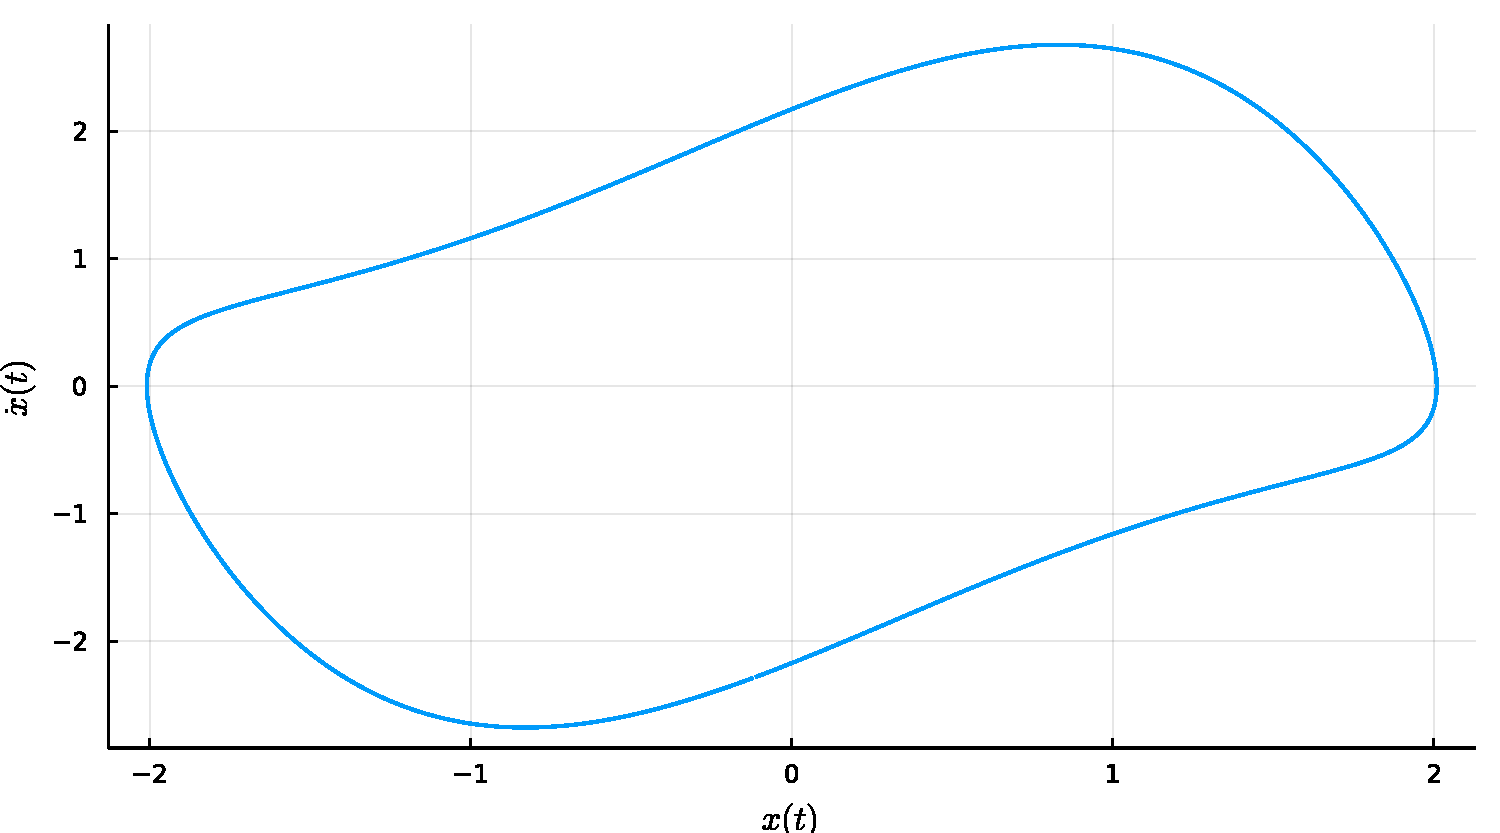
\includegraphics[keepaspectratio,scale = 0.35]{05_ODE/Phase_plot.pdf}
	\caption{Newton法で求めた周期解の位相図\newline \qquad (横軸:$x(t)$, 縦軸:$\dot{x}(t)$)}
	\label{fig:Phase_plot}
	\end{center}
\end{figure}

\begin{figure}[h]
	\centering
	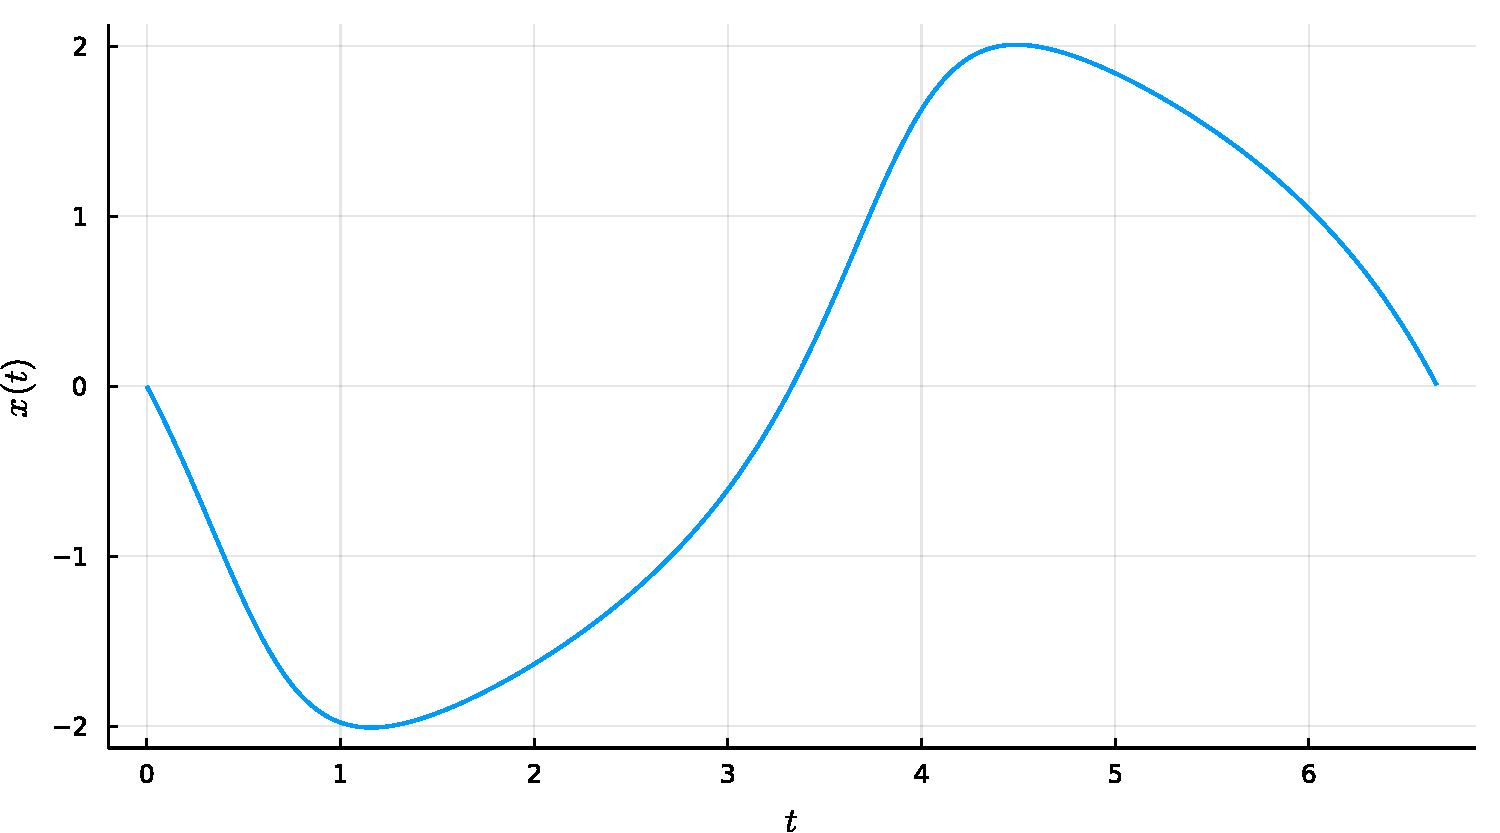
\includegraphics[keepaspectratio,scale = 0.35]{05_ODE/solution.pdf}
	\caption{周期解のプロファイル(横軸:$t$, 縦軸:$x(t)$)}
	\label{fig:solution}
\end{figure}

\begin{figure}[h]
	\centering
	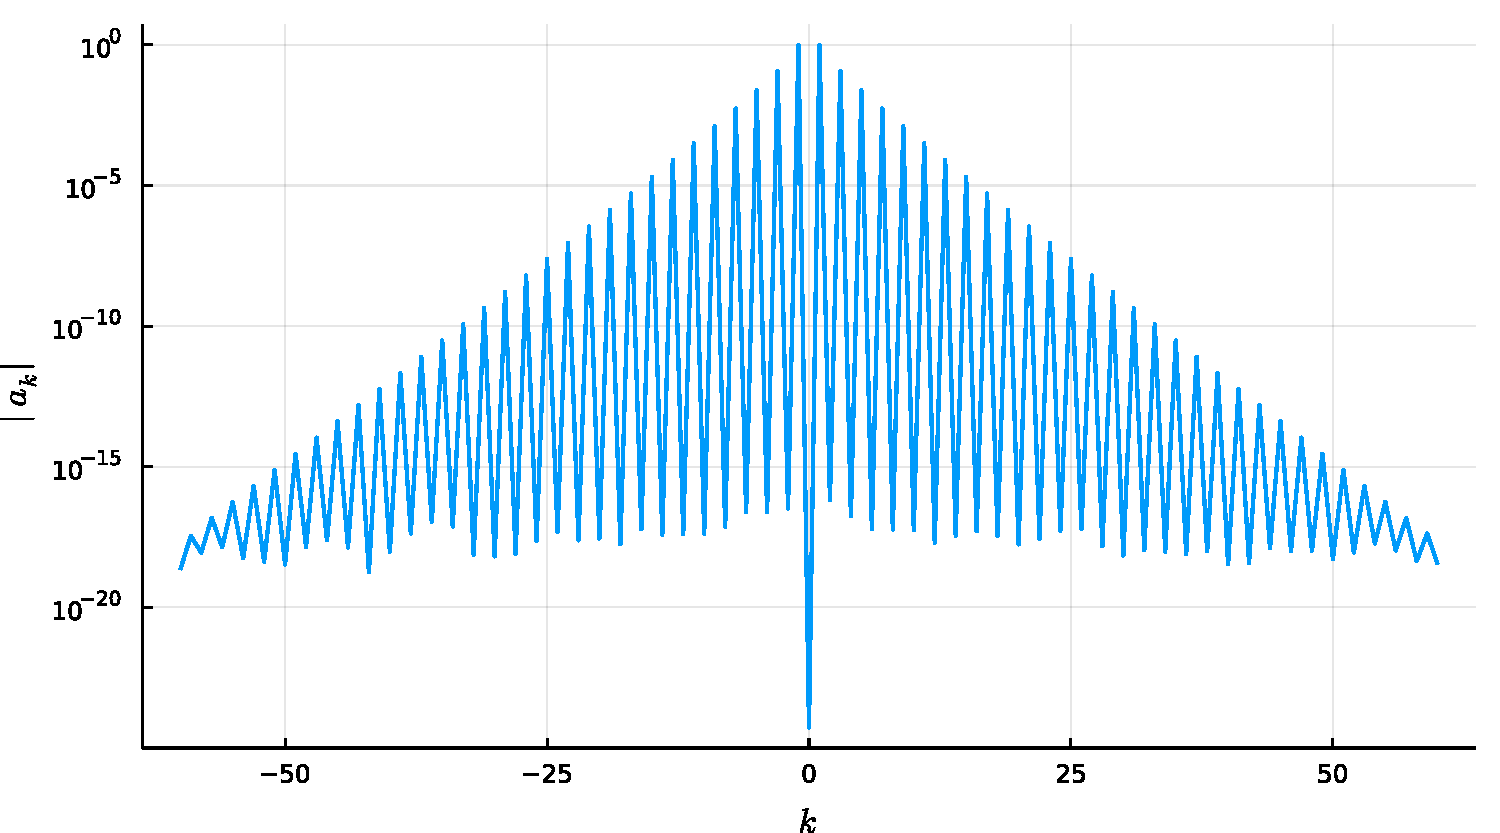
\includegraphics[keepaspectratio,scale = 0.35]{05_ODE/coeffs.pdf}
	\caption{近似周期解のフーリエ係数}
	\label{fig:coeffs}
\end{figure}

\clearpage

フーリエ係数の図を見ると、係数が $10^{-18}$ 程度まで落ちていることがわかり、高精度に近似解を求められていることが期待される。



%\end{document}}
\newcommand{\VerifyPO}{%!TEX root = ../main.tex

%\documentclass[twoside,twocolumn,a4j,dvipdfmx]{jarticle}
%\usepackage{amsmath,amssymb}
%\usepackage[dvipdfmx]{graphicx}
%\newcommand{\im}{\mathrm{i}}
%\newcommand{\bx}{\mathrm x}
%\newcommand{\R}{\mathbb{R}}
%\newcommand{\Largezero}{\mbox{\Large{0}}}
%\newcommand{\Hugezero}{\mbox{\Huge{0}}}
%\newtheorem{thm}{定理}[section]
%\newtheorem{df}[thm]{定義}
%\newtheorem{lem}{補助定理}[section]
%\newtheorem{prop}[thm]{補題}
%\setcounter{MaxMatrixCols}{100}

%\begin{document}
この章では、van der Pol方程式
$$
\frac{d^2 x}{dt^2} - \mu (1-x^2)\frac{dx}{dt} + x = 0
$$
の周期解の数値検証方法の詳細を記し、精度保証を行う。

\subsection{作用素$A^\dagger$ , $A$ の定義}

\subsubsection{$A^\dagger$ の定義}

Banach空間 $X= \mathbb{C} \times \ell^1_\nu, Y=\mathbb{C} \times \ell^1_{\nu'}$ ($\nu'<\nu$) と設定し、$A^\dagger$ を $A^\dagger \in \mathcal{L}(X,Y)$ として、$b=(b_0,b_1)\in \mathbb{C}\times \ell^1_\nu = X$に対して、 $A^\dagger b = ((A^\dagger b)_0 , (A^\dagger b)_1 )$ と作用するように定義する。ここで、 $A^\dagger$ を形式的に見ると、
\footnotesize
\begin{align*}
    A^\dagger &= 
    \left[\begin{array}{c|cccccc}
    0 & 1 &  \cdots  & 1 & \cdots & {0} & \cdots  \\\hline
    \vdots & &  \vdots & & & & \\
    \partial_\omega f_k & \cdots & \partial_{a_j} f_k & \cdots & & \Hugezero &\\
    \vdots& &  \vdots & & & & \\
    \vdots & & & & \lambda_N & & \Largezero   \\
    0 & & \Hugezero & & & \lambda_{N+1} & \\
    \vdots & & & & \Largezero& & \ddots
    \end{array}\right] \\
    &=
    \left[
    \begin{array}{c|c}
    0 & A_{a,0}^\dagger \\
    \hline 
    A_{\omega, 1}^\dagger & A_{a,1}^\dagger
    \end{array}
    \right].
\end{align*}
\normalsize
このことから、 $A^\dagger b$ は、
    \begin{align*}
    A^\dagger b &= 
    \begin{bmatrix}
    0 & A_{a,0}^\dagger \\
    A_{\omega ,1}^\dagger & A_{a,1}^\dagger
    \end{bmatrix}
    \times
    \begin{bmatrix}
    b_0 \\
    b_1
    \end{bmatrix} \\
    &=
    \begin{bmatrix}
    A^\dagger_{a,0} b_1 \\
    A^\dagger_{\omega ,1} b_0 + A^\dagger_{a,1} b_1
    \end{bmatrix}
    =: 
    \begin{bmatrix}
    (A^\dagger b)_0 \\
    (A^\dagger b)_1
    \end{bmatrix}
    \end{align*}
と表すことができ、
$$
    (A^\dagger b)_0 = \sum_{|k|<N} (b_1)_k
$$
\footnotesize
\begin{align*}
    ((A^\dagger b)_1 )_k &:= 
    \begin{cases}
    \partial_\omega f_k b_0 + \sum_{|j|<N} \partial_{a_j} f_k (b_1 )_j, &|k| < N  \\
    \lambda_k (b_1)_k &|k| \ge N
    \end{cases} \\
    \lambda_k &:= -k^2 \omega^2 - \mu \im k \omega + 1
\end{align*}
\normalsize
と具体的に書ける。またこのとき、$(A^\dagger b)_0$と$(A^\dagger b)_1$はそれぞれ
    \begin{align*}
    (A^\dagger b)_0 = A^\dagger_{a,0} b_1 = \sum_{|k|<N} (b_1)_k \in \mathbb{C} \\
    (A^\dagger b)_1 = A^\dagger_{\omega, 1} b_0 + A^\dagger_{a,1} b_1 \in \ell^1_{\nu^\prime}.
    \end{align*}

\begin{rem}
上のtail部分は実際には添字$k$に対して正負両方の向きに伸びているが、今回は一方向のみ表記している。
\end{rem}

\subsubsection{$A$ の定義}

次に作用素 $A$ について考える。 
$$
    A^{(N)} = 
    \begin{bmatrix}
    A_{\omega,0}^{(N)} & A_{a,0}^{(N)} \\
    A_{\omega,1}^{N)} & A_{a,1}^{(N)}
    \end{bmatrix}
    \approx DF^{(N)}(\bar{\bx})^{-1} \in \mathbb{C}^{2N \times 2N}
$$
をJacobi行列の近似逆行列とする。そして、$A \in \mathcal{L}(Y,X)$ として、$b = (b_0, b_1 ) \in X$に対して、 $Ab = ((Ab)_0, (Ab)_1)$ と作用するように定義する。ここで、
    \begin{align*}
    (Ab)_0 &= A_{\omega,0}^{(N)}b_0 + A_{a,0}^{(N)}b_1^{(N)} \\
    (Ab)_1 &= A_{\omega,1}^{(N)}b_0 + A_{a,1}b_1.
    \end{align*}
ただし、無限次元の $A_{a,1}b_1$ は以下のようになる。
$$
    (A_{a,1} b_1 )_k = 
    \begin{cases}
    (A_{a,1}^{(N)}b_1^{(N)})_k &(|k| < N) \\
    (b_1)_k / \lambda_k &(|k| \ge N).
    \end{cases}
$$
この定義を形式的に見ると
\begin{align*}
    A &=
    \left[
    \begin{array}{c|cccc}
    A^{(N)}_{\omega , 0} & A^{(N)}_{a,0} & 0 & \cdots & 0 \\
    \hline
    A^{(N)}_{\omega ,1} & A^{(N)}_{a,1} &  & \Largezero &\\
    0 & &\frac1{\lambda_{N}} &  & \\
    \vdots & & & \frac1{\lambda_{N+1}} & \\
    0 & & \Largezero & & \ddots
    \end{array}
    \right]\\
    &=
    \left[
    \begin{array}{c|c}
    0 & A_{a,0} \\
    \hline 
    A_{\omega, 1} & A_{a,1}
    \end{array}
    \right].
\end{align*}
と表記できる。

\subsection{$Y_0, Z_0, Z_1, Z_2$ の評価}

\subsubsection{$Y_0$の評価}
今、
$$
    F(\bar \bx) = (\delta_0 , \delta_1) \in \mathbb{C} \times \ell^1_{\nu'}
$$
とすると、$A$の定義より、
\begin{align*}
    \|AF(\bar \bx)\|_X \leq \max&\Biggl\{|A^{(N)}_{\omega, 0} \delta_0 + A^{(N)}_{a,0} \delta^{(N)}_1|,  \\
    &~ \left. \|A^{(N)}_{\omega,1} \delta_0 + A_{a,1} \delta^{(N)}_1 \|_{w} \right. \\
    &~ + \sum_{|k| > N} \left| \frac{(\delta^{\infty}_1)_k}{\lambda_k} \right| \nu^{|k|}\Biggr\}=:Y_0.
\end{align*}
ここで、$\delta_1=(\delta_1^{(N)}, \delta^{(\infty)}_1)\in\mathbb{C}^{2*3(N-1)+1}$であり、
$$
    (\delta_1)_k = 
    \begin{cases}
    \delta_1^{(N)} &(k < |N|) \\
    \delta_1^{(\infty)} &(k \geq |N|)
    \end{cases}
$$
と表した。

\subsubsection{$Z_0$の評価}
次に、 $Z_0$ の評価を与える。
$$
    % \begin{align*}
    B := I - AA^\dagger = \begin{bmatrix}
          B_{\omega , 0} & B_{a,0} \\
          B_{\omega, 1} & B_{a,1}
         \end{bmatrix}.
    % \end{align*}
$$
この $B$ を $c \in \overline{B(0,1)}, \| c \|_X \le 1$ である $c = (c_0, c_1)$ に作用させると、
    \begin{align*}
    (Bc)_0 &= B_{\omega,0} c_0 + B_{a,0}c_1 \\
    (Bc)_1 &= B_{\omega,1} c_0 + B_{a,1}c_1.
    \end{align*}
ここで、$(Bc)_0$ はスカラ値なので、
\begin{align*}
|B_{a,0} c_1| &\leq \sum_{k \in \mathbb{Z}}|(B_{a,0})_k||(c_1)_k| \\
&= \sum_{k \in \mathbb{Z}} \frac{|(B_{a,0})_k|}{w_k} |(c_1)_k|w_k \\
&\leq \underset{k < |N|}{\max} \frac{|(B_{a,0})_k|}{w_k} \sum_{k \in \mathbb{Z}} |(c_1)_k|w_k \\
&\leq \underset{k < |N|}{\max} \frac{|(B_{a,0})_k|}{w_k}, \\
&(\sum_{k \in \mathbb{Z} }|(c_1)_k|w_k = \|c_1 \|_w \le 1).
\end{align*}
よって、
$$
|(Bc)_0| \leq |B_{\omega,0}| + \underset{|k| < N}{\max} \frac{|(B_{a,0})_k|}{\omega_k} = Z_0^{(0)}.
$$
またここで、作用素 $M:\ell_{\nu}^1\to \ell_{\nu}^1$ の作用素ノルムについて以下の補題を準備する。

\begin{prop}
行列 $M^{(N)}$ を $M^{(N)} \in \mathbb{C}^{(2N-1) \times (2N-1)}$ 、双方向の複素無限点列(a bi-infinite sequence of complex numbers) を $\{ \delta_k \}_{|k| \geq N}$ と定義する。ここで、 $\delta_N > 0$ であり、
$$
    |\delta_k| \leq \delta_N \text{ for all } |k| \geq N.
$$
を満たすとする。そして、$a = (a_k)_{k \in \mathbb{Z}} \in \ell^1_\nu$ に対して 
$a^{(N)} = (a_{-N+1} , \dots, a_{N-1}) \in \mathbb{C}^{2N-1}$と表し、
作用素 $M:\ell_{\nu}^1\to \ell_{\nu}^1$ を以下のように定義する。
$$
    [Ma]_k := 
    \begin{cases}
    [M^{(N)}a^{(N)}]_k, & |k| < N \\
    \delta_k a_k ,& |k| \geq N.
    \end{cases}
$$
このとき、 $M$ は有界線形作用素であり、
\begin{align*}
    \|M\|_{\mathcal{L}(\ell^1_\nu)} &\leq \max{(K,\delta_N)},\\
    K &:= \max_{|n|<N} \frac{1}{\nu^{|n|}} \sum_{|k|<N} |M_{k,n}| \nu^{|k|}
\end{align*}
と評価される。
\end{prop}

上の補題を利用すると、
$$
    \| (Bc)_1 \|_w \leq \| B_{\omega,1} \|_w + \| B_{a,1} \|_{\mathcal{L}(\ell_\nu^{1})} = Z_0^{(1)}
$$
が評価可能となり、結論としては、求めたい $Z_0$ は $Z_0 := \{Z_0^{(0)}, Z_0^{(1)}\}$ となる。

\subsubsection{$Z_1$ の評価}
さらに $Z_1$ の評価を与える。 $Z_1$ は次の不等式を満たす。
\begin{align*}
    \|A(DF(\bar{\bx}) - A^\dagger ) c \|_X &\leq Z_1,\\
\mbox{ここで, }    c = (c_0, c_1) \in \overline{B(0,1)} \Leftrightarrow \|c \|_X &\leq 1.
\end{align*}
点列 $z$ を下記のように定義する。
$$
    z := (DF(\bar{\bx}) - A^\dagger ) c = 
    \begin{bmatrix}
    z_0 \\
    z_1
    \end{bmatrix}.
$$
ここで、$DF(\bar{\bx})$ と $A^\dagger$ は
$$
    DF(\bar{\bx}) =
    \left[\begin{array}{c|ccc}
    0 & \cdots & 1 & \cdots \\\hline
    \vdots & &\vdots&\\
    \partial_{\omega}f_k& \dots & \partial_{a_j}f_k & \dots\\
    \vdots & &\vdots& 
    \end{array}\right],
$$
\footnotesize
$$
    A^\dagger =
    \left[
    \begin{array}{c|cccccc}
    0 & \cdots & \partial_a \eta & \cdots & 0 & \cdots & 0 \\
    \hline
    \vdots &  & \vdots & & & & \\
    \partial_\omega f_{k}^{(N)} & \cdots & \partial_{a_j} f_{k}^{(N)} & \cdots & & & \\
    \vdots & & \vdots & & \Large{0} & \\
    0 & & & \lambda_{N} & & & \\
    \vdots & & & & \lambda_{N+1} & & \\
    0 & & \Large{0} & & & \ddots
    \end{array}
    \right],
$$
\normalsize
$$
    \lambda_k := -k^2 \omega^2 - \mu \im k \omega + 1
$$
と表される。すると $z_0$ は、
$$
    z_0 = \sum_{|k| \ge N} (c_1 )_k, |z_0| \leq \frac{1}{w_{N}} \sum_{|k| \ge N} |(c_1)_k| w_k \leq \frac{1}{w_{N}}.
$$

次に、 $z_1$ について考える。 $DF(\bar{\bx})c$ 部分は
    \begin{align*}
    ((DF(\bar{\bx})c)_1)_k &= \partial_\omega f_k c_0 + \partial_a f_k c_1 \\
    &= \frac{\partial \lambda_k}{\partial \omega} c_0 \bar{a}_k + \frac{\mu \im k}{3}(\bar{a} * \bar{a} * \bar{a})_k c_0 \\
    & ~+ \lambda_k (c_1)_k + \mu \im k \omega (\bar{a} * \bar{a} * c_1)_k, \\
    &\quad k \in \mathbb{Z}
    \end{align*}
と書け、 $|k| \geq N$ で $\bar{a}_k = 0$ より、 $c_1 = c_1^{(N)} + c_1^{(\infty)}$ として、

\footnotesize
$$
    (z_1)_k = 
    \begin{cases}
    \mu \im k \omega (\bar{a} * \bar{a} * c_1^{(\infty)})_k , ~ |k| < N\\
    \frac{\mu \im k}{3}(\bar{a} * \bar{a} * \bar{a})_k c_0 + \mu \im k \omega (\bar{a} * \bar{a} * c_1)_k, ~ |k| \geq N
    \end{cases}
$$
\normalsize
と表せる。ここから、 $z_1$ の絶対値をとると、 $|k| < N$ で
\begin{align*}
    |(z_1)_k| \leq |\mu \im k \omega| \max
    &\left\{ 
    \max_{k-N+1 \leq j \leq -N} \frac{|(\bar{a} * \bar{a})_{k-j}|}{w_j}, \right. \\
    &~~ \left. \max_{N \leq j \leq k+N-1} \frac{|(\bar{a} * \bar{a})_{k-j}|}{w_j}
    \right\} \\
    &=:\zeta,\quad \zeta = (\zeta_k)_{|k| < N} \in \mathbb{R}^{2N-1}.
\end{align*}

最後に、 $Z_1$ を求める。 $Z_1^{(0)}$ は次を満たすとする。
    \begin{align*}
    |(A(DF(\bar{\bx}) - A^\dagger)c)_0| &= |(Az)_0| \\
    &\leq |A_{\omega,0}^{(N)}| |z_0| + |A_{a,0}^{(N)}| | z_1^{(N)}| \\
    &\leq \frac{|A_{\omega,0}^{(N)}|}{w_{N}} + |A_{a,0}^{(N)}|\zeta \\
    &=: Z_1^{(0)}.
    \end{align*}
そして、$Z_1^{(1)}$ は次を満たすとする。
\footnotesize
    \begin{align*}
    \|(A(DF(\bar{\bx}) - A^\dagger)c)_1 \|_w &= \|(Az)_1 \|_w \\
    &= \| A_{\omega,1}^{(N)} z_0 + A_{a,1} z_1 \|_w \\
    &\leq \frac{\|A_{\omega,1}^{(N)} \|_w}{w_{N}} + \sum_{|k|<N} (|A_{a,1}^{(N)}| \zeta)_k w_k \\
    &~~+ \sum_{|k| \geq N} \frac{|\mu \im k (\bar{a}*\bar{a}*\bar{a})_k |}{3|\lambda_k |} w_k  \\
    &~~+ \sum_{|k| \geq N} \frac{ |\mu \im k \omega ( \bar{a} * \bar{a} * c_1 )_k |}{|\lambda_k|} w_k \\
    &\leq \frac{\|A_{\omega,1}^{(N)} \|_w}{w_{N}} + \sum_{|k|<N} (|A_{a,1}^{(N)}| \zeta)_k w_k\\
    &~~+ \sum_{N\le |k| \le 3(N-1)} \frac{|\mu \im k (\bar{a}*\bar{a}*\bar{a})_k |}{3|\lambda_k |} w_k  \\
    &~~+ \sum_{|k| \geq N} \frac{ |\mu \im k \omega ( \bar{a} * \bar{a} * c_1 )_k |}{|\lambda_k|} w_k \\
    &\leq \frac{\| A_{\omega,1}^{(N)} \|_w}{w_{N}} + \| |A_{a,1}^{(N)}| \zeta \|_w \\
    &~~+ \sum_{N\le |k| \le 3(N-1)} \frac{|\mu \im k (\bar{a}*\bar{a}*\bar{a})_k |}{3|\lambda_k |} w_k  \\
    &~~+ \frac{1}{N} \frac{\mu \omega \|\bar{a} \|_{w}^2}{\omega^2 - \frac{1}{N^2}} \\
    &=: Z_1^{(1)}.
    \end{align*}
\normalsize

よって、
$$
    Z_1 := \max\{Z_1^{(0)}, Z_1^{(1)}\}.
$$

\textbf{$Z_1^{(1)}$ の評価の補足}

上の評価に現れる
$$
\sum_{|k| \geq N} \frac{ |\mu \im k \omega ( \bar{a} * \bar{a} * c_1 )_k |}{|\lambda_k|} w_k \\
$$
は、$\lambda_k := -k^2 \omega^2 - \mu \im k \omega + 1$ より、次で評価される。
\footnotesize
\begin{align*}
\sum_{|k| \geq N} \frac{ |\mu \im k \omega ( \bar{a} * \bar{a} * c_1 )_k |}{|\lambda_k|} w_k 
&= \sum_{|k| \geq N} \frac{ |\mu \im k \omega ( \bar{a} * \bar{a} * c_1 )_k |}{|-k^2 \omega^2 - \mu \im k \omega + 1|} w_k \\
&\leq \sum_{|k| \geq N} \frac{1}{|k|} \frac{ |\mu \im \omega ( \bar{a} * \bar{a} * c_1 )_k |}{|\omega^2 + \frac{\mu \im \omega}{k} - \frac{1}{k^2}|} w_k \\
&\leq \sum_{|k| \geq N} \frac{1}{|k|} \frac{ |\mu \im \omega ( \bar{a} * \bar{a} * c_1 )_k |}{|\omega^2 - \frac{1}{k^2}|} w_k \\
&\leq \frac{1}{N} \frac{\mu \im \omega \|\bar{a} \|_{w}^2}{\omega^2 - \frac{1}{N^2}}.
\end{align*}
\normalsize

\subsubsection{$Z_2$ の評価}
最後に $Z_2$ の評価を与える。今、
$b \in \overline{B(\bar{\bx},r)}, c = (c_0, c_1) \in \overline{B(0,1)}$ について、 $Z_2$ の評価は次の不等式を満たす。
$$
    \| A(DF(b) - DF(\bar{\bx}))c \|_X \leq Z_2 (r)r
$$
まず $z$ を、
$$
    z := (DF(b) - DF(\bar{\bx}))c = 
    \begin{bmatrix}
    z_0 \\
    z_1 \\
    \end{bmatrix}
    =
    \begin{bmatrix}
    0 \\
    z_1 \\
    \end{bmatrix}
$$
と定義する。 $DF$ の定義から $z_0 = 0$ となるので、 $z_1$ だけを考えればよく、
\begin{align*}
    (z_1)_k := &(\partial_\omega f_k (b) - \partial_\omega f_k (\bar{\bx})) c_0 \\
     &+ [(\partial_a f(b) - \partial_a f(\bar{\bx}))c_1]_k , k \in \mathbb{Z}
\end{align*}
と書ける。$b = (\omega, (a_k)_{k \in \mathbb{Z}}), \bar{\bx} = (\bar{\omega}, (\bar{a}_k)_{|k| < N})$ として、第1項は、
    \begin{align*}
    &(\partial_\omega f_k (b) - \partial_\omega f_k (\bar{\bx}))c_0 \\
    &= \left[((- 2 k^2 \omega - \mu \im k)a_k + \frac{\mu \im k}{3} (a*a*a)_k) \right.\\
    &~~~\left. - (( - 2 k^2 \bar{\omega} - \mu \im k) \bar{a}_k + \frac{\mu \im k}{3}(\bar{a}*\bar{a}*\bar{a})_k)\right]c_0 \\
    &= \left[ -2k^2 \omega (a_k - \bar{a}_k) - 2 k^2 (\omega - \bar{\omega}) \bar{a}_k - \mu \im k (a_k - \bar{a_k}) \right.\\
    &\left. ~~~+ \frac{\mu \im k}{3}((a*a*a)_k - (\bar{a}*\bar{a}*\bar{a})_k) \right] c_0
    \end{align*}
と書ける。そして、第2項は、
    \begin{align*}
    &[(\partial_a f(b) - \partial_a f(\bar{\bx}))c_1]_k \\
    &= (-k^2 \omega^2 - \mu \im k \omega +1)(c_1)_k + \mu \im k \omega (a*a*c_1)_k -\\
    &~~~[(-k^2 \bar{\omega}^2 - \mu \im k \bar{\omega} +1)(c_1)_k + \mu \im k \bar{\omega} (\bar{a}*\bar{a}*c_1)_k] \\
    &= [ -k^2 (\omega + \bar{\omega})(\omega - \bar{\omega}) - \mu \im k (\omega - \bar{\omega})](c_1)_k \\
    &~~~+ \mu \im k \omega ((a+\bar{a})*(a-\bar{a})*c_1)_k \\
    &~~~+ \mu \im k (\omega - \bar{\omega}) (\bar{a}*\bar{a}*c_1)_k
    \end{align*}
と書ける。$(Az)_0, (Az)_1$ は、
\begin{align*}
    (Az)_0 &= A_{a,0}^{(N)} z_1^{(N)} \\
    (Az)_1 &= A_{a,1}z_1
\end{align*}
より、
$$
    \| Az \|_X = \max \left\{ |A_{a,0}^{(N)}z_1^{(N)}|, \| A_{a,1}z_1 \|_w \right\}
$$
となる。

次に、$|A_{a,0}^{(N)}z_1^{(N)}|$ を上から評価する。はじめに、$\tilde{A}_{a,0},\tilde{B}_{a,0}$ を以下のように定義する。
\begin{align*}
    \tilde{A}_{a,0} := (|k| (A_{a,0}^{(N)})_k )_{|k| < N} \\
    \tilde{B}_{a,0} := (k^2 (A_{a,0}^{(N)})_k )_{|k| < N}.
\end{align*}
すると、
\begin{align*}
|A_{a,0}^{(N)}z_1^{(N)}| &\leq 2 (\bar{\omega} + r) \|\tilde{B}_{a,0}\|_{w^*} r + 2 \|\tilde{B}_{a,0}\|_{w^*} \|\bar{a}\|_w r \\
    &\quad + \mu \|\tilde{A}_{a,0}\|_{w^*} r \\
    &\quad + \frac{\mu}{3} \|\tilde{A}_{a,0}\|_{w^*} (r^2 + 3 \|\bar{a}\|_w r + 3 \|\bar{a}\|^2_w )r \\
    &\quad + \|\tilde{B}_{a,0}\|_{w^*} (2 \bar{\omega} + r) r + \mu \|\tilde{A}_{a,0}\|_{w^*} r \\
    &\quad + \mu (\bar{\omega} + r) \|\tilde{A}_{a,0}\|_{w^*} (2 \|\bar{a}\|_w + r) r \\
    &\quad + \mu \|\tilde{A}_{a,0}\|_{w^*} \|\bar{a}\|^2_w r \\
    &= Z_2^{(4,0)} r^3 + Z_2^{(3,0)} r^2 + Z_2^{(2,0)} r
\end{align*}
となる。同様に $\| A_{a,1} z_1 \|_w$ を上から評価する。$\tilde{A}_{a,1},\tilde{B}_{a,1}$ を以下のように定義する。
\begin{align*}
    \tilde{A}_{a,1} := (|j| (A_{a,1})_{k,j} )_{k,j \in \mathbb{Z}} \\
    \tilde{B}_{a,1} := (j^2 (A_{a,1})_{k,j} )_{k,j \in \mathbb{Z}}.
\end{align*}
すると、 
\begin{align*}
    \| A_{a,1} z_1 \|_w &\leq  2 (\bar{\omega} + r) \|\tilde{B}_{a,1}\|_{\mathcal{L}(\ell^1_\nu)} r + 2 \|\tilde{B}_{a,1}\|_{\mathcal{L}(\ell^1_\nu)} \|\bar{a}\|_w r \\
   &\quad + \mu \|\tilde{A}_{a,1}\|_{\mathcal{L}(\ell^1_\nu)} r \\
   &\quad+ \frac{\mu}{3} \|\tilde{A}_{a,1}\|_{\mathcal{L}(\ell^1_\nu)} (r^2 + 3 \|\bar{a}\|_w r + 3 \|\bar{a}\|^2_w )r \\
   &\quad + \|\tilde{B}_{a,1}\|_{\mathcal{L}(\ell^1_\nu)} (2 \bar{\omega} + r) r + \mu \|\tilde{A}_{a,1}\|_{\mathcal{L}(\ell^1_\nu)} r \\
   &\quad+ \mu (\bar{\omega} + r) \|\tilde{A}_{a,1}\|_{\mathcal{L}(\ell^1_\nu)} (2 \|\bar{a}\|_w + r) r \\
   &\quad + \mu \|\tilde{A}_{a,1}\|_{\mathcal{L}(\ell^1_\nu)} \|\bar{a}\|^2_w r \\
    &= Z_2^{(4,1)} r^3 + Z_2^{(3,1)} r^2 + Z_2^{(2,1)} r
\end{align*}
と書ける。 上記の$Z_2^{(4,1)},Z_2^{(3,1)},Z_2^{(2,1)}$ は、先ほどの$\tilde{A}_{a,0},\tilde{B}_{a,0}$ を $\tilde{A}_{a,1},\tilde{B}_{a,1}$ に置き換えて、適切なノルム評価をしたものになる。

最終的に、 $j = 2,3,4$ で
$$
    Z_2^{(j)} := \max \{ Z_2^{(j,0)} , Z_2^{(j,1)} \}
$$
とすれば、
$$
    Z_2(r) = Z_2^{(4)} r^2 + Z_2^{(3)} r + Z_2^{(2)} 
$$
となる。

\subsection{radii polynomial の精度保証}

上で求めた各評価を用いて、radii polynomial を以下で構成する。
$$
    p(r) := Z_2 (r)r^2 - (1 - Z_1 - Z_0)r + Y_0.
$$
そして、$p(r_0)<0$ となる$r_0>0$ を求める。各評価の計算は、Juliaの \texttt{IntervalArithmetic.jl} を用いて区間演算を行っており、それぞれの評価の上界(sup) を用いて $r_0$ の区間を求めた。この $r_0$ の検証手法は、まず、各評価の上界を代入した $p(r)$ をNewton法反復により、$p(\bar r) \approx 0$ となる$r_0$ の近似解を求め、これを基に $r_0$ を含む区間をKrawczyk法で検証する。\cite{radiipolynomial_interval}

\subsubsection{各評価の上界の値と区間$r_0$}
各評価の上界の値と区間 $r_0$ は以下の値になった。
\begin{align*}
Y_0 &= 2.1648276355041128 \times 10^{-7} \\
Z_0 &= 1.9782535732448317 \times 10^{-11} \\
Z_1 &= 0.19932204092542252 \\
Z_2^{(2)} &= 69.97604726405831 \\
Z_2^{(3)} &= 26.652787246376946 \\
Z_2^{(4)} &= 2.390949473898198 \\
r_0 &= [2.7038 \times 10^{-7},  2.70381 \times 10^{-7}]
\end{align*}

そして、 $p(r)$ のグラフは以下のようになった。

\begin{figure}[h]
	\centering
	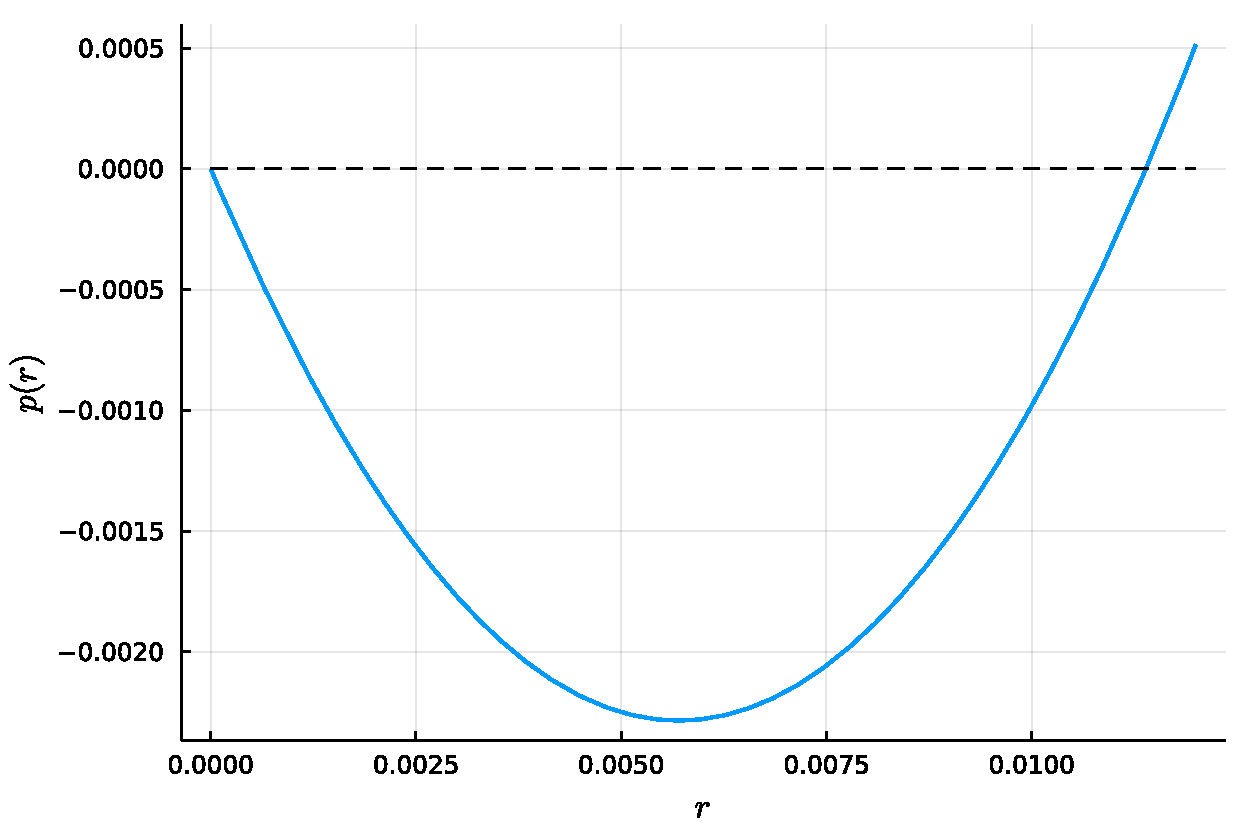
\includegraphics[keepaspectratio,scale = 0.35]{./06_VerifyPO/radii_polynomial.pdf}
	\caption{radii polynomial の概形}
\end{figure}

このことから、フーリエスペクトル法とNewton法の反復によって得た近似解の近傍 $\overline{B(\bar{\bx},r)}$ 内に $F(\bar{\bx}) = 0$ となる $\bar{\bx}$ が一意存在し、この$\bar{\bx}$ は、van der Pol方程式の周期解となる。

%\end{document}}
\newcommand{\Conclusion}{%!TEX root = ../main.tex
%\documentclass[twoside,twocolumn,a4j,dvipdfmx]{jarticle}
%\usepackage{amsmath,amssymb}
%\usepackage[dvipdfmx]{graphicx}
%\newcommand{\im}{\mathrm{i}}
%\newcommand{\bx}{\mathrm x}
%\newcommand{\R}{\mathbb{R}}
%\newcommand{\Largezero}{\mbox{\Large{0}}}
%\newcommand{\Hugezero}{\mbox{\Huge{0}}}
%\newtheorem{thm}{定理}[section]
%\newtheorem{df}[thm]{定義}
%\newtheorem{lem}{補助定理}[section]
%\newtheorem{prop}[thm]{補題}
%\setcounter{MaxMatrixCols}{100}

%\begin{document}
%\section{おわりに}
本研究では、van der Pol方程式の周期解をフーリエ級数で表現し、フーリエ係数に対する零点探索問題を考えることで、Newton Kantorovich型定理の成立を数値検証した。今後の展望は、JuliaとMATLAB上の区間演算パッケージINTLABとの計算コストの比較を行い、Juliaの有用性を検証したい。また、他の方程式についてもJuliaで実装していきたい。
%\end{document}}

%theorem
\newtheorem{thm}{定理}[section]
\newtheorem{df}[thm]{定義}
\newtheorem{lem}{補助定理}[section]
\newtheorem{prop}[thm]{補題}
\newtheorem{example}[thm]{例}
\newtheorem{rem}[thm]{注意}

%caption
\captionsetup[figure]{font = small}

%
%%%%%% ここから論文内容 %%%%%%
%
% 次の行には、000000の代わりに自分の学籍番号を、KOUSHISUの
% 代わりに大文字のローマ字で自分の名字を例にならって書いて
% 下さい。
%
\pagestyle{myheadings}
%\markboth{\it 000000 KOSHISU}{\it 000000 KOUSHISU}
\esysid{201811134 TAKAHASHI}
%
%
% 題目を書いて下さい
%
\title{{\Large Julia言語を用いた常微分方程式の周期解の精度保証付き数値計算} \\ {\large Rigorous numerics for periodic solutions of ODEs using Julia language}}
%
% 著者名、著者名のローマ字表記、指導教員名を例にならって書い
% て下さい
%
\author{{\Large 高橋 和暉 } \\ KAZUKI TAKAHASHI \\ (指導教員  高安 亮紀)}

%
% 卒業論文の概要を書いて下さい
%
\eabstract{On the one hand, numerical computation is an efficient technique for solving mathematical problems including various differential equations numerically. On the other hand, one cannot avoid errors in numerical computing. Rigorous numerics is a method to evaluate the error of numerical computations rigorously and to derive mathematically rigorous results. It should be an efficient tool for controlling risks in numerical computations. In this study, using the Julia language, we implement a method of rigorous numerics for periodic solutions of the van der Pol equation. In particular, we approximate the periodic solution by a Fourier series and numerically validate the hypothesis of the Newton-Kantorovich type theorem by considering a zero-finding problem for the Fourier coefficients.
}

\begin{document}

\begin{titlepage}
\begin{center}
\vspace*{10mm}
{\large 令和三年度 筑波大学工学システム学類卒業研究論文} \\
\vspace*{30mm}
{\Large Julia言語を用いた常微分方程式の周期解の精度保証付き数値計算} 
\vspace{100mm} \\
\begin{tabular}{rl}
{\Large 学籍番号} & {\Large 201811134} \\
\addlinespace[10mm]
{\Large 氏名} & {\Large 高橋 和暉} \\
\addlinespace[10mm]
{\Large 指導教員} & {\Large 高安 亮紀}
\end{tabular} 
\end{center}
\end{titlepage}

\clearpage

\maketitle
\thispagestyle{headings}

\section{はじめに}
\Introduction

\section{Fourier級数}
\Fourierseries

\section{離散畳み込み(Discrete Convolution)}
\Convolution

\section{周期解の精度保証付き数値計算の諸理論}
\Theories

\section{van der Pol方程式の周期解の数値計算}
\ODE

\section{van der Pol方程式の周期解の精度保証}
\VerifyPO

\section{おわりに}
\Conclusion

\section{謝辞}
指導教員の高安亮紀先生から大変丁寧なご指導を賜りました。厚く感謝を申し上げます。また、同研究室の遠藤靖典先生からも大変丁寧なご指導を賜りました。厚く感謝を申し上げます。さらに、同研究室の皆様からも大変多くのご助言を頂きました、厚く感謝を申し上げます。

\begin{thebibliography}{99}
\bibitem{seidohoshou}
大石進一, 『精度保証付き数値計算の基礎』, コロナ社, 2018.

\bibitem{convolution}
Jean-Phileppe Lessard. Computing discrete convolutions with verified accuracy via Banach algebras and the FFT. Applications of Mathematics, 63(3):219–235, 2018.

\bibitem{radiipolynomial}
Jean-Philippe Lessard, Jason Mireles James, Julian Ransford, Automatic differentiation for Fourier series and the radii polynomial approach. Physica D  Nonlinear Phenomena 334(299), 2016.

\bibitem{JPLessard}
Jean-Philippe Lessard. Continuation of solutions and studying delay differential equations via rigorous numerics. In Jan Bouwe van den Berg and Jean-Philippe Lessard, editors, Rigorous numerics in dynamics, pages 81-122, Providence, Rhode Island, 2018. American Mathematical Society.
\bibitem{FFT}
井藤佳奈子, 高安亮紀, Juliaで精度保証付き高速フーリエ変換, \url{https://www.risk.tsukuba.ac.jp/~takitoshi/tutorial/verifyfft.html}, 2021.

\bibitem{DEjl}
DifferentialEquations.jl: Scientific Machine Learning (SciML) Enabled Simulation and Estimation, \url{https://diffeq.sciml.ai/stable/}, 2021.

\bibitem{radiipolynomial_interval}
大谷俊輔, 高安亮紀,Juliaで非線型方程式の解の精度保証付き数値計算, \url{https://www.risk.tsukuba.ac.jp/~takitoshi/tutorial/verifynlss.html}, 2020.

\end{thebibliography}

\end{document}
